\subsection{Evidencia modular: mecanismos y límites}
\label{sec:evidencia-modular-sintesis}

A0--FULL responde la pregunta integrada; SP1--SP8 explican por qué falla cada abstracción cuando se estudia por separado. Esta sección conserva de cada campaña solo la formulación mínima necesaria, el resultado que cambia la interpretación y el límite que impide generalizarlo. Los algoritmos, configuraciones, tablas completas y manifiestos permanecen en los artefactos reproducibles citados en el Anexo~\ref{sec:reproducibilidad}.

\subsubsection{De la preferencia continua a la factibilidad mecánica: SP1--SP3}

\paragraph{SP1: reclutamiento homogéneo y efecto del cierre.}
\label{sec:resultados-sp1-homogeneous}
SP1 reúne el emparejamiento uno a uno ($q=1$) y el reclutamiento por cuórum ($q>1$). Cada robot mantiene una preferencia $x_i\in\Delta^K$ y comparte el potencial
\[
 \Phi(x)=-\frac{\alpha}{2}\sum_k\bigl(n_k(x)-q\bigr)^2
         -\beta\sum_{i,k}c_{ik}x_{ik}.
\]
Smith, replicator y BNN usan el gradiente del mismo potencial; el cierre QR transforma después la preferencia continua en una coalición entera. Esta separación permite atribuir por separado la dinámica, la decodificación y la factibilidad.

La campaña abarcó 900 mundos emparejados. Smith+QR redujo el regret frente a \emph{greedy} en $0{,}0212$ (IC95\% $[-0{,}0284,-0{,}0141]$), pero la subasta proxy lo mejoró en $0{,}0299$ y uniforme+QR en $0{,}0153$. Con información completa, el regret de Smith fue $0{,}0117$; con cuatro rondas de consenso en anillo aumentó a $0{,}1076$. La auditoría verificó invariancia del símplex y ascenso de potencial, pero el cierre QR observa preferencias globales y no demuestra distribución de extremo a extremo.

\begin{figure}[tbp]
\centering
\begin{minipage}[t]{0.49\textwidth}
\centering
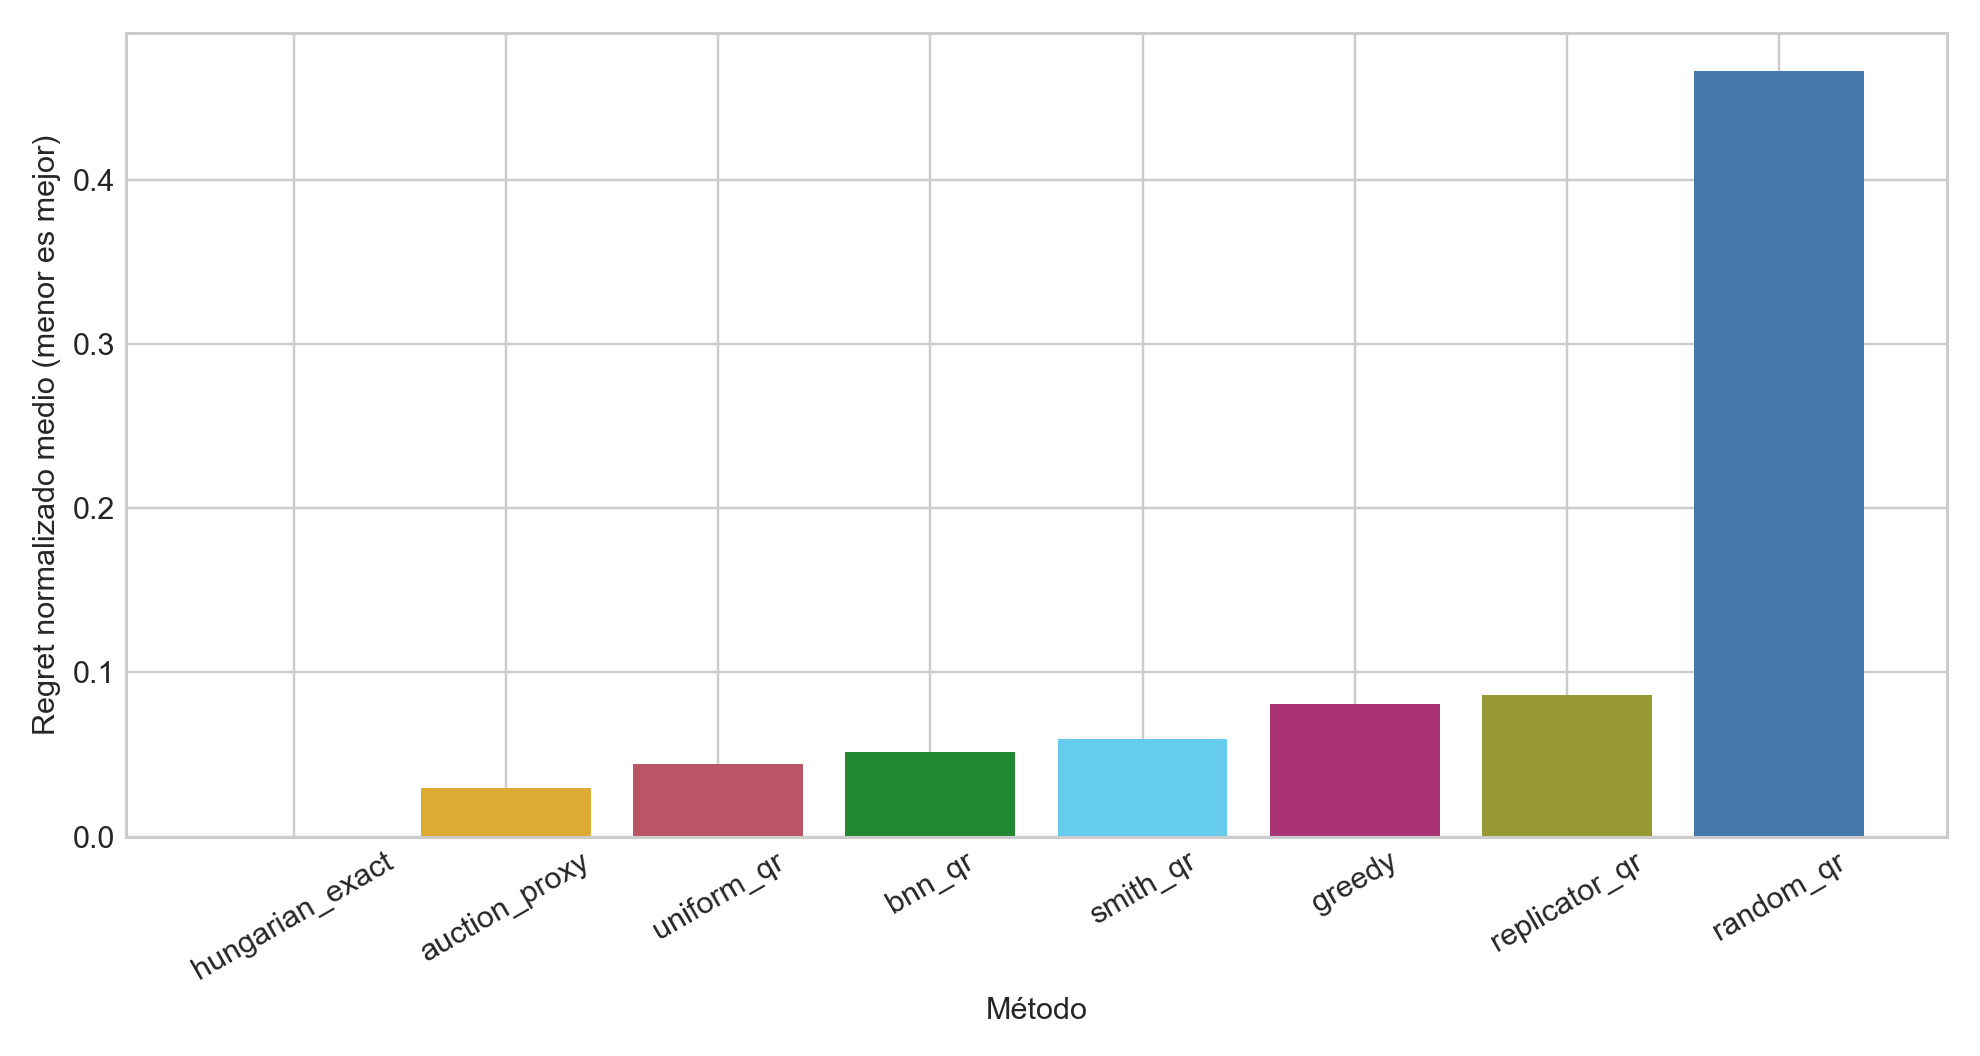
\includegraphics[width=\linewidth]{figures/fig-sp1-homogeneous-regret.png}
\end{minipage}\hfill
\begin{minipage}[t]{0.49\textwidth}
\centering
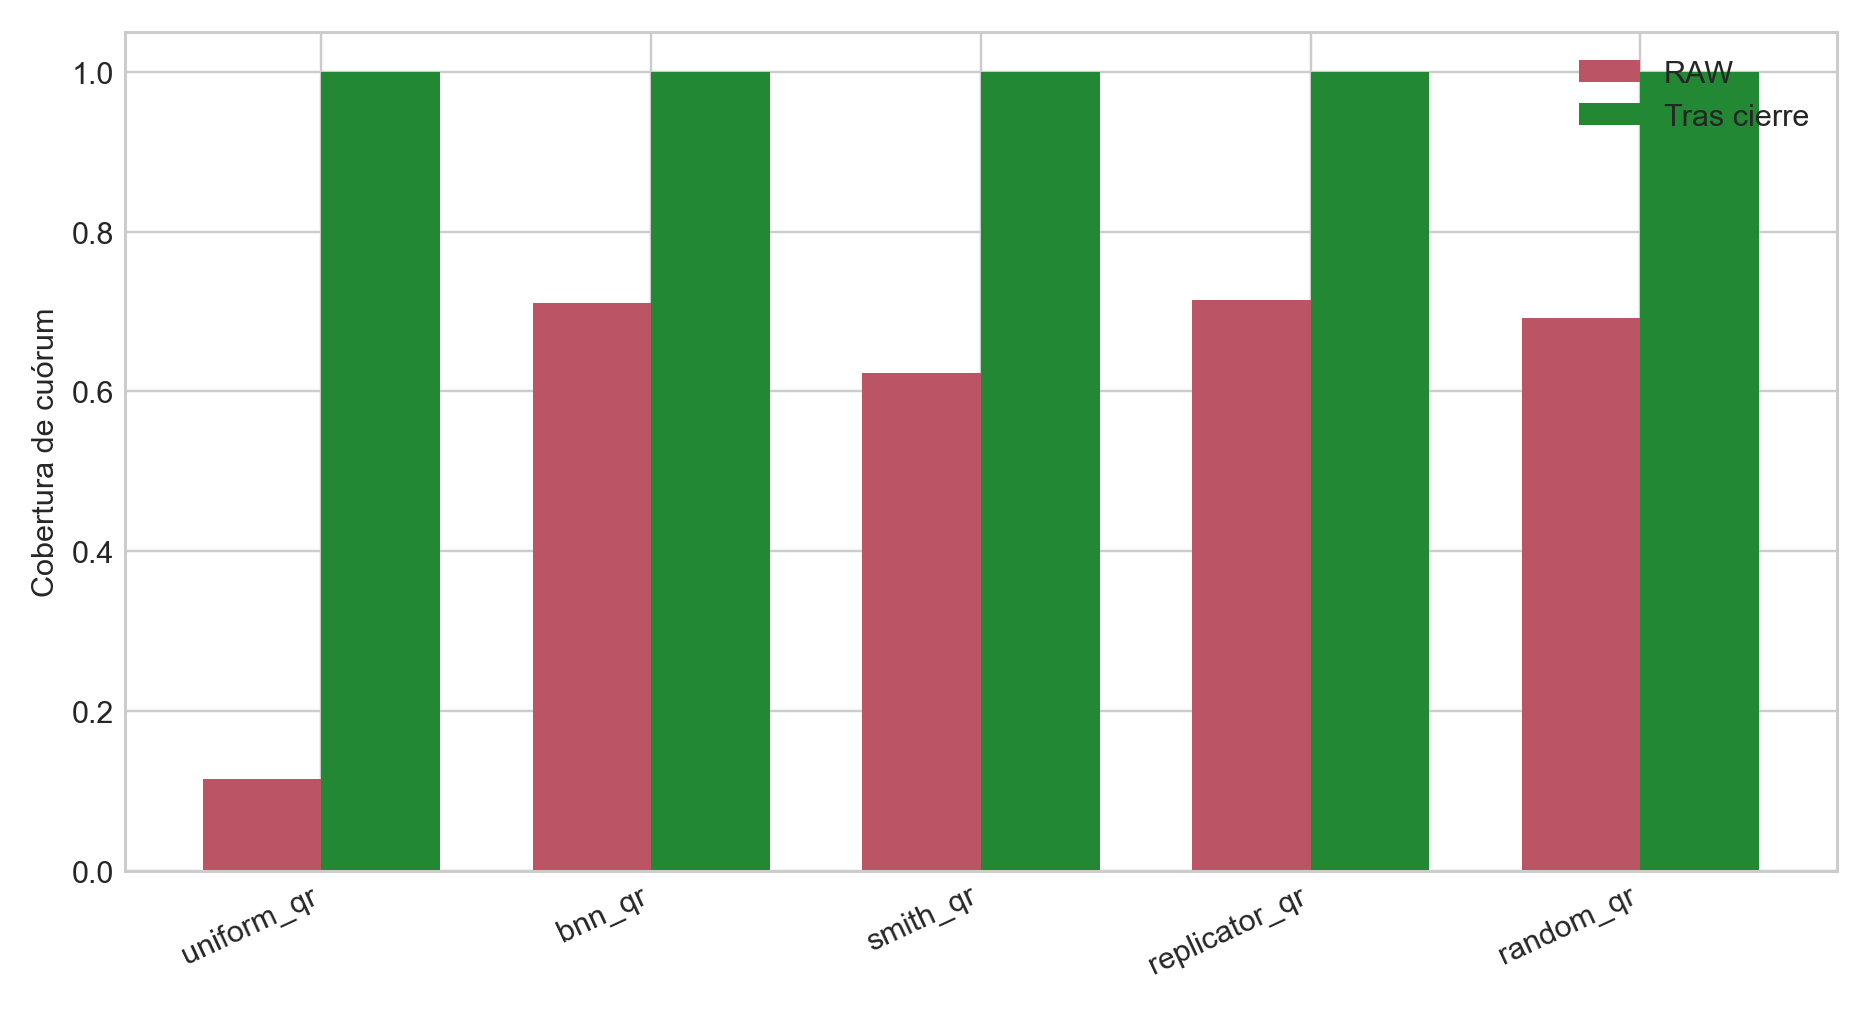
\includegraphics[width=\linewidth]{figures/fig-sp1-homogeneous-raw-closed.png}
\end{minipage}
\caption[Resultado decisivo de SP1]{SP1 separa la calidad de la preferencia continua (RAW) del efecto del cierre entero (CLOSED) en 900 mundos.}
\viuownsource
\label{fig:sp1-homogeneous-main}
\end{figure}

El control uniforme contiene la conclusión decisiva: una parte sustancial de la calidad procede del cierre y no del motor poblacional. SP1 respalda la formulación continua y su trazabilidad; no establece optimalidad entera ni superioridad general de Smith.

\paragraph{SP2: capacidad efectiva y separación entre fitness y protocolo.}
SP2 sustituye el conteo de robots por una contribución robot--carga $e_{ik}=c_i\eta_{ik}$. La capacidad agregada,
\[
 S_k(x)=\sum_i e_{ik}x_{ik},
\]
entra en el gradiente marginal del juego. Smith, replicator y ERV--BNN reciben el mismo fitness, y todas las preferencias se cierran con el mismo decodificador de capacidad. El diseño factorial comprueba así si la mejora procede de la señal física, del protocolo de revisión o del cierre.

En 480 mundos, los fitness marginales redujeron el regret frente al déficit \emph{plain}: $-0{,}0264$ para Smith, $-0{,}0178$ para replicator y $-0{,}0338$ para ERV--BNN. Bajo la variante logarítmica no apareció un protocolo ganador; las diferencias entre ERV--BNN, Smith y replicator incluyeron cero. ERV--BNN+log mejoró a \emph{greedy} en $0{,}0504$, pero el MILP conservó una ventaja de $0{,}2880$.

\begin{figure}[tbp]
\centering
\begin{minipage}[t]{0.49\textwidth}
\centering
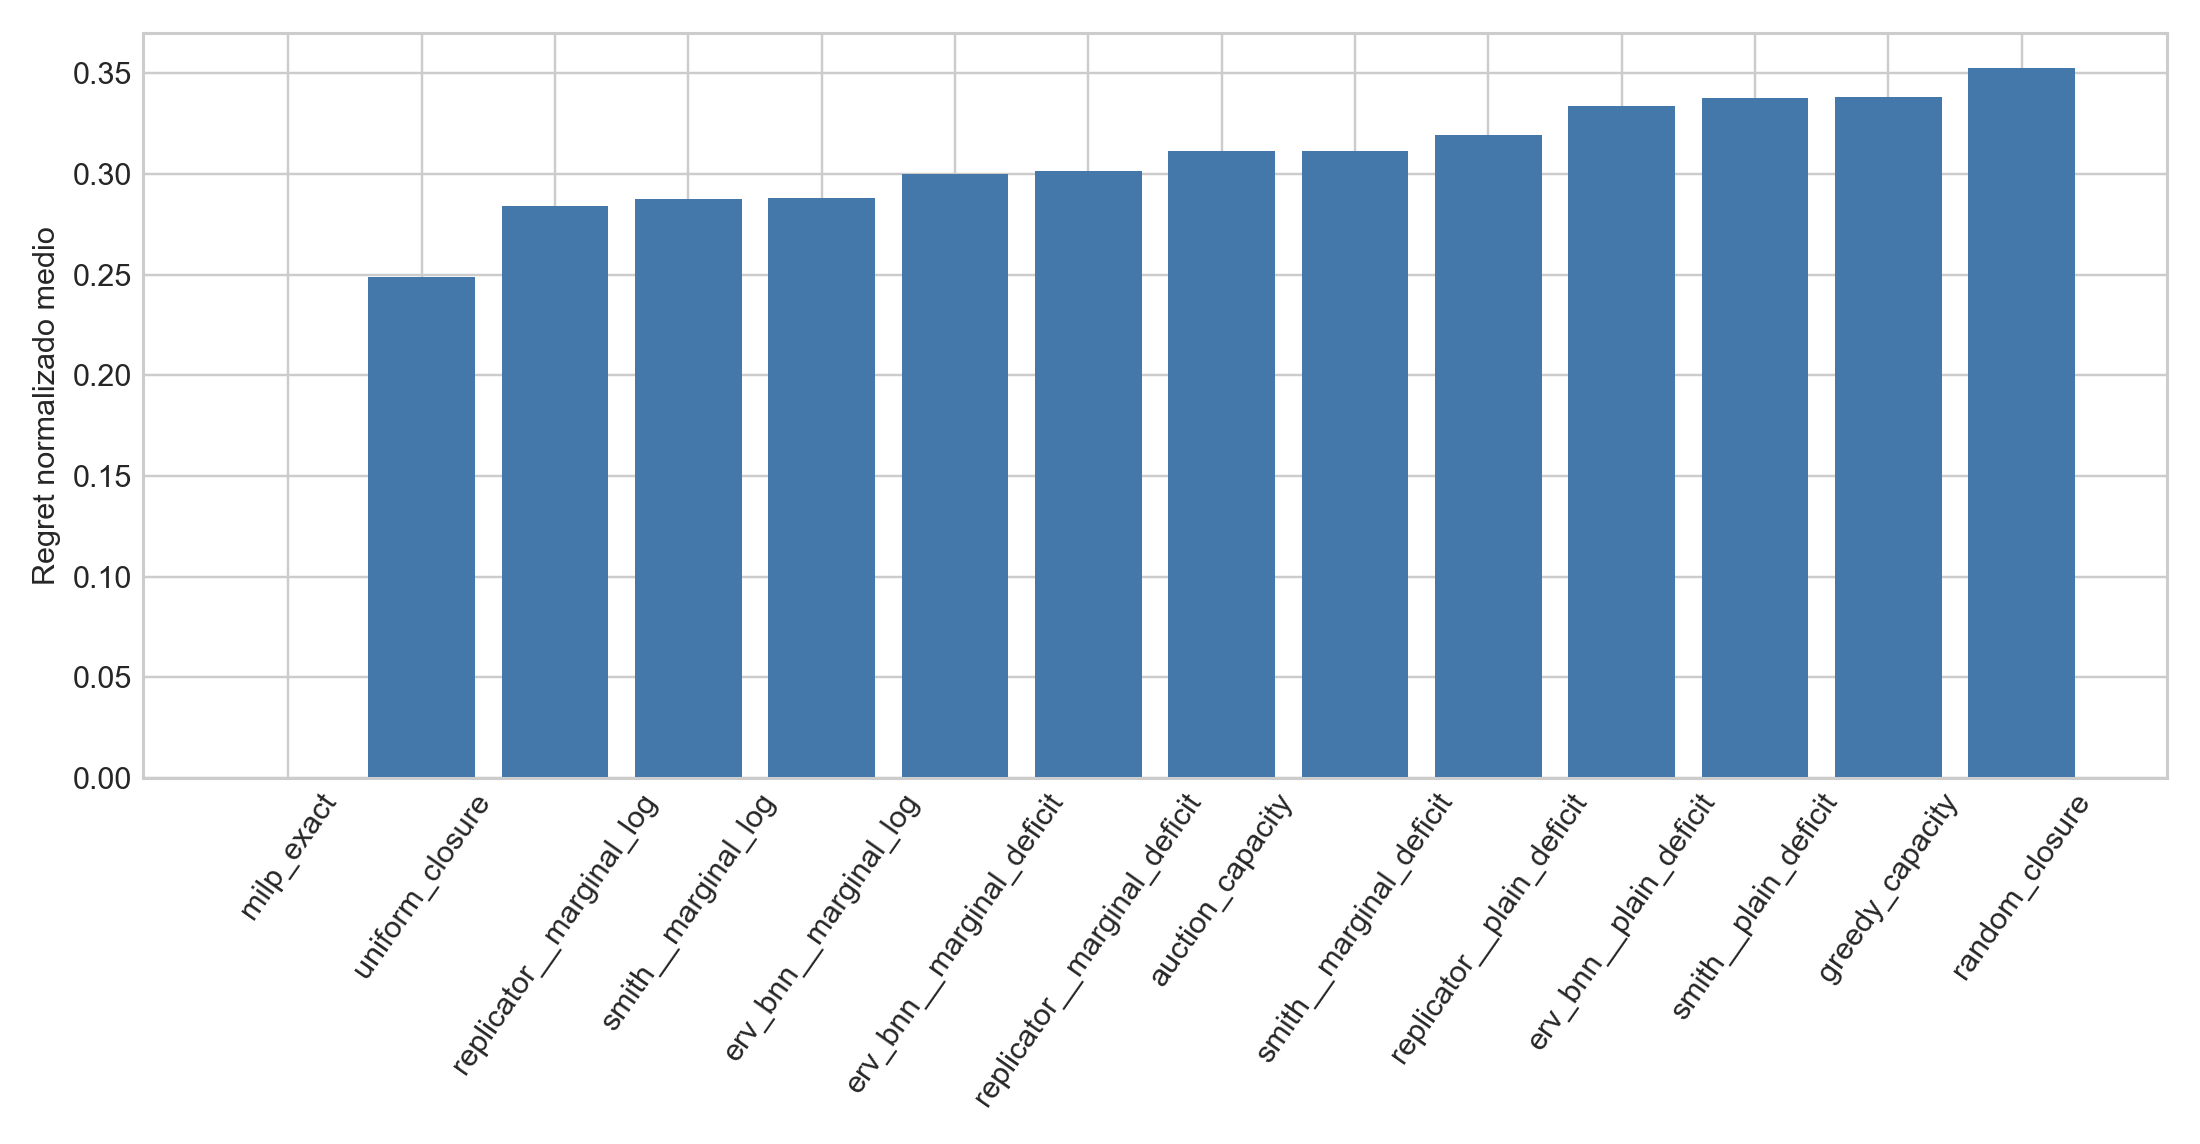
\includegraphics[width=\linewidth]{figures/fig-sp2-heterogeneous-regret.png}
\end{minipage}\hfill
\begin{minipage}[t]{0.49\textwidth}
\centering
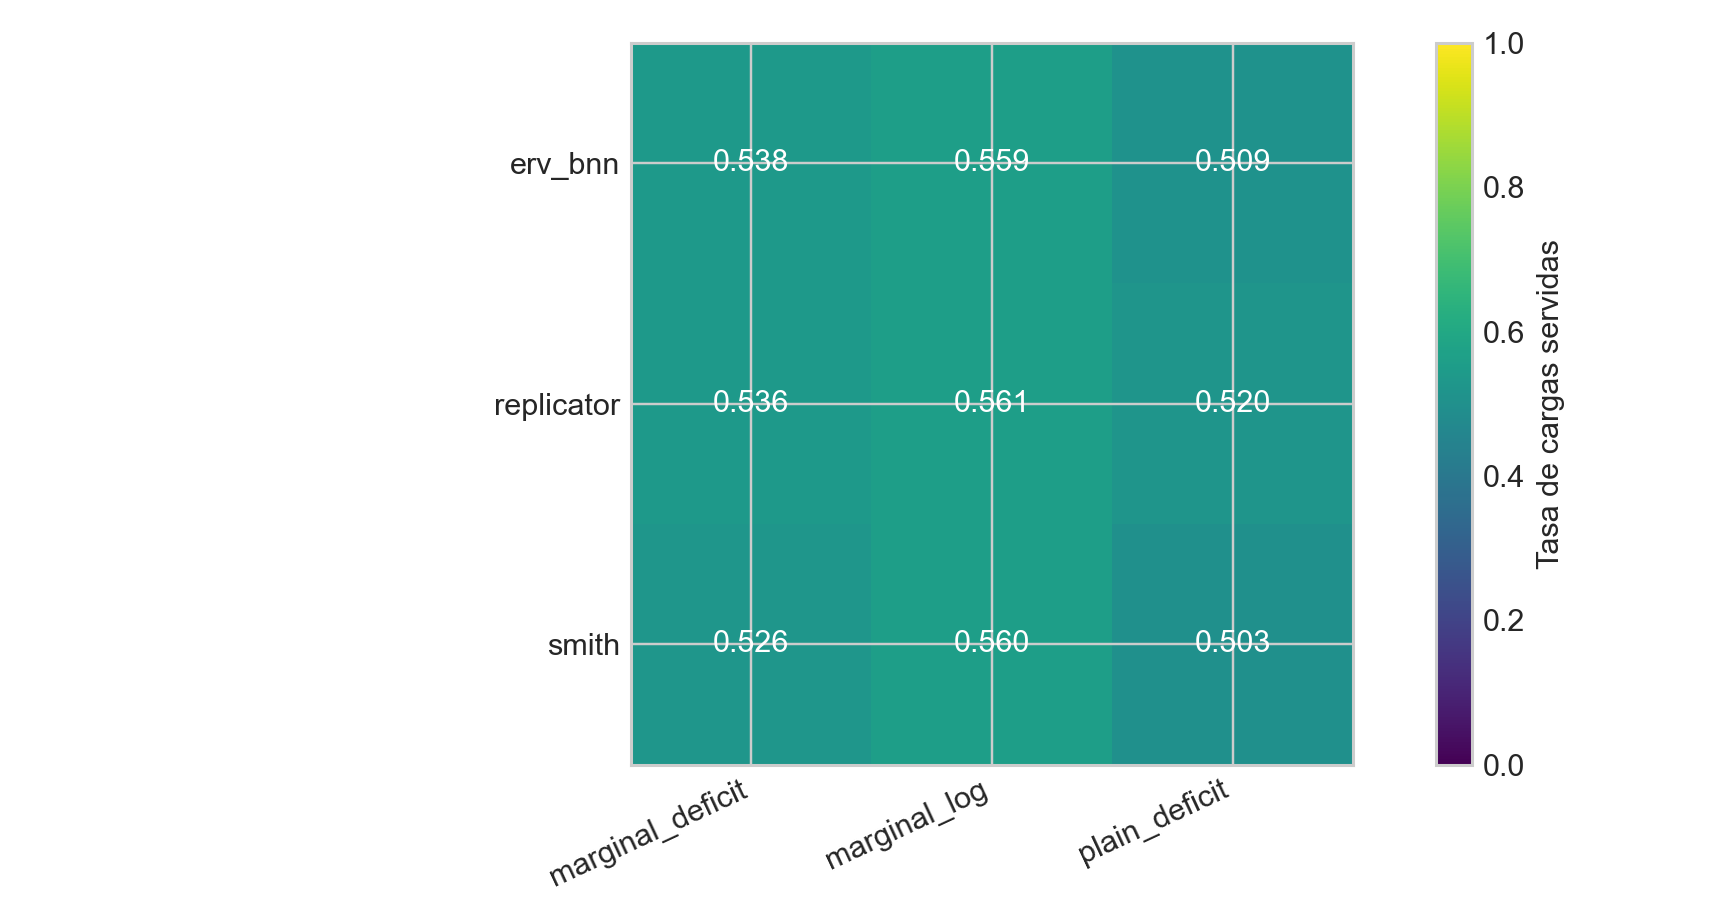
\includegraphics[width=\linewidth]{figures/fig-sp2-fitness-protocol.png}
\end{minipage}
\caption[Resultado factorial de SP2]{SP2 muestra el regret por método y la interacción entre fitness y protocolo de revisión.}
\viuownsource
\label{fig:sp2-heterogeneous-main}
\end{figure}

El resultado más informativo fue negativo: uniforme+closure alcanzó regret $0{,}2489$, menor que las nueve variantes de juego. El cierre pasó de cero cargas servidas en RAW a $0{,}5994$ después de usar capacidad marginal y distancia. Por tanto, SP2 demuestra que la capacidad debe entrar en la decisión, pero también que el decodificador aporta información suficiente para dominar la preferencia poblacional en esta campaña. Además, $e_{ik}$ sigue siendo escalar y no acredita fuerza y torque; esa frontera motiva SP3.

\paragraph{SP3: contactos y factibilidad \emph{wrench}.}
SP3 incorpora la geometría que SP2 omite. Para una coalición $S$, el residual normalizado es
\[
 \rho_S(w)=
 \frac{\min_{0\leq f\leq\bar f}\lVert G_Sf-w\rVert_2}
      {\max(\lVert w\rVert_2,\varepsilon)}.
\]
Para la relajación continua, los simplex locales y las restricciones acopladas son
convexos. Si existe un punto de Slater y la regularización es estrictamente positiva,
las KKT son necesarias y suficientes para el óptimo del potencial; al compartir el
multiplicador de la restricción acoplada, ese punto coincide con el v-GNE. La equivalencia
no se extiende al cierre entero ni a la guardia global
\citep{yi2019operator,cherukuri2016primaldual}.
La relajación continua usa precios de fuerza, torque y ocupación de slots; el cierre resuelve conflictos enteros y una guardia añade robots individuales o pares hasta satisfacer el residual. La guardia observa la geometría completa y los robots libres, por lo que se declara global.

La campaña v1.1 reunió 600 mundos y 7.200 ejecuciones. Projected primal--dual con información exacta alcanzó brecha máxima de potencial $0{,}00339$ frente al QP y residual KKT medio $0{,}00221$. Sin guardia, su tasa de falsos positivos fue $0{,}3333$; la guardia la redujo a cero (IC95\% para la diferencia $[-0{,}3700,-0{,}2950]$). El criterio escalar, \emph{greedy wrench} y CBBA aceptaron indebidamente $0{,}5000$ de los casos condicionados, lo que confirma dentro del generador que capacidad escalar y factibilidad \emph{wrench} son constructos distintos.

\begin{figure}[tbp]
\centering
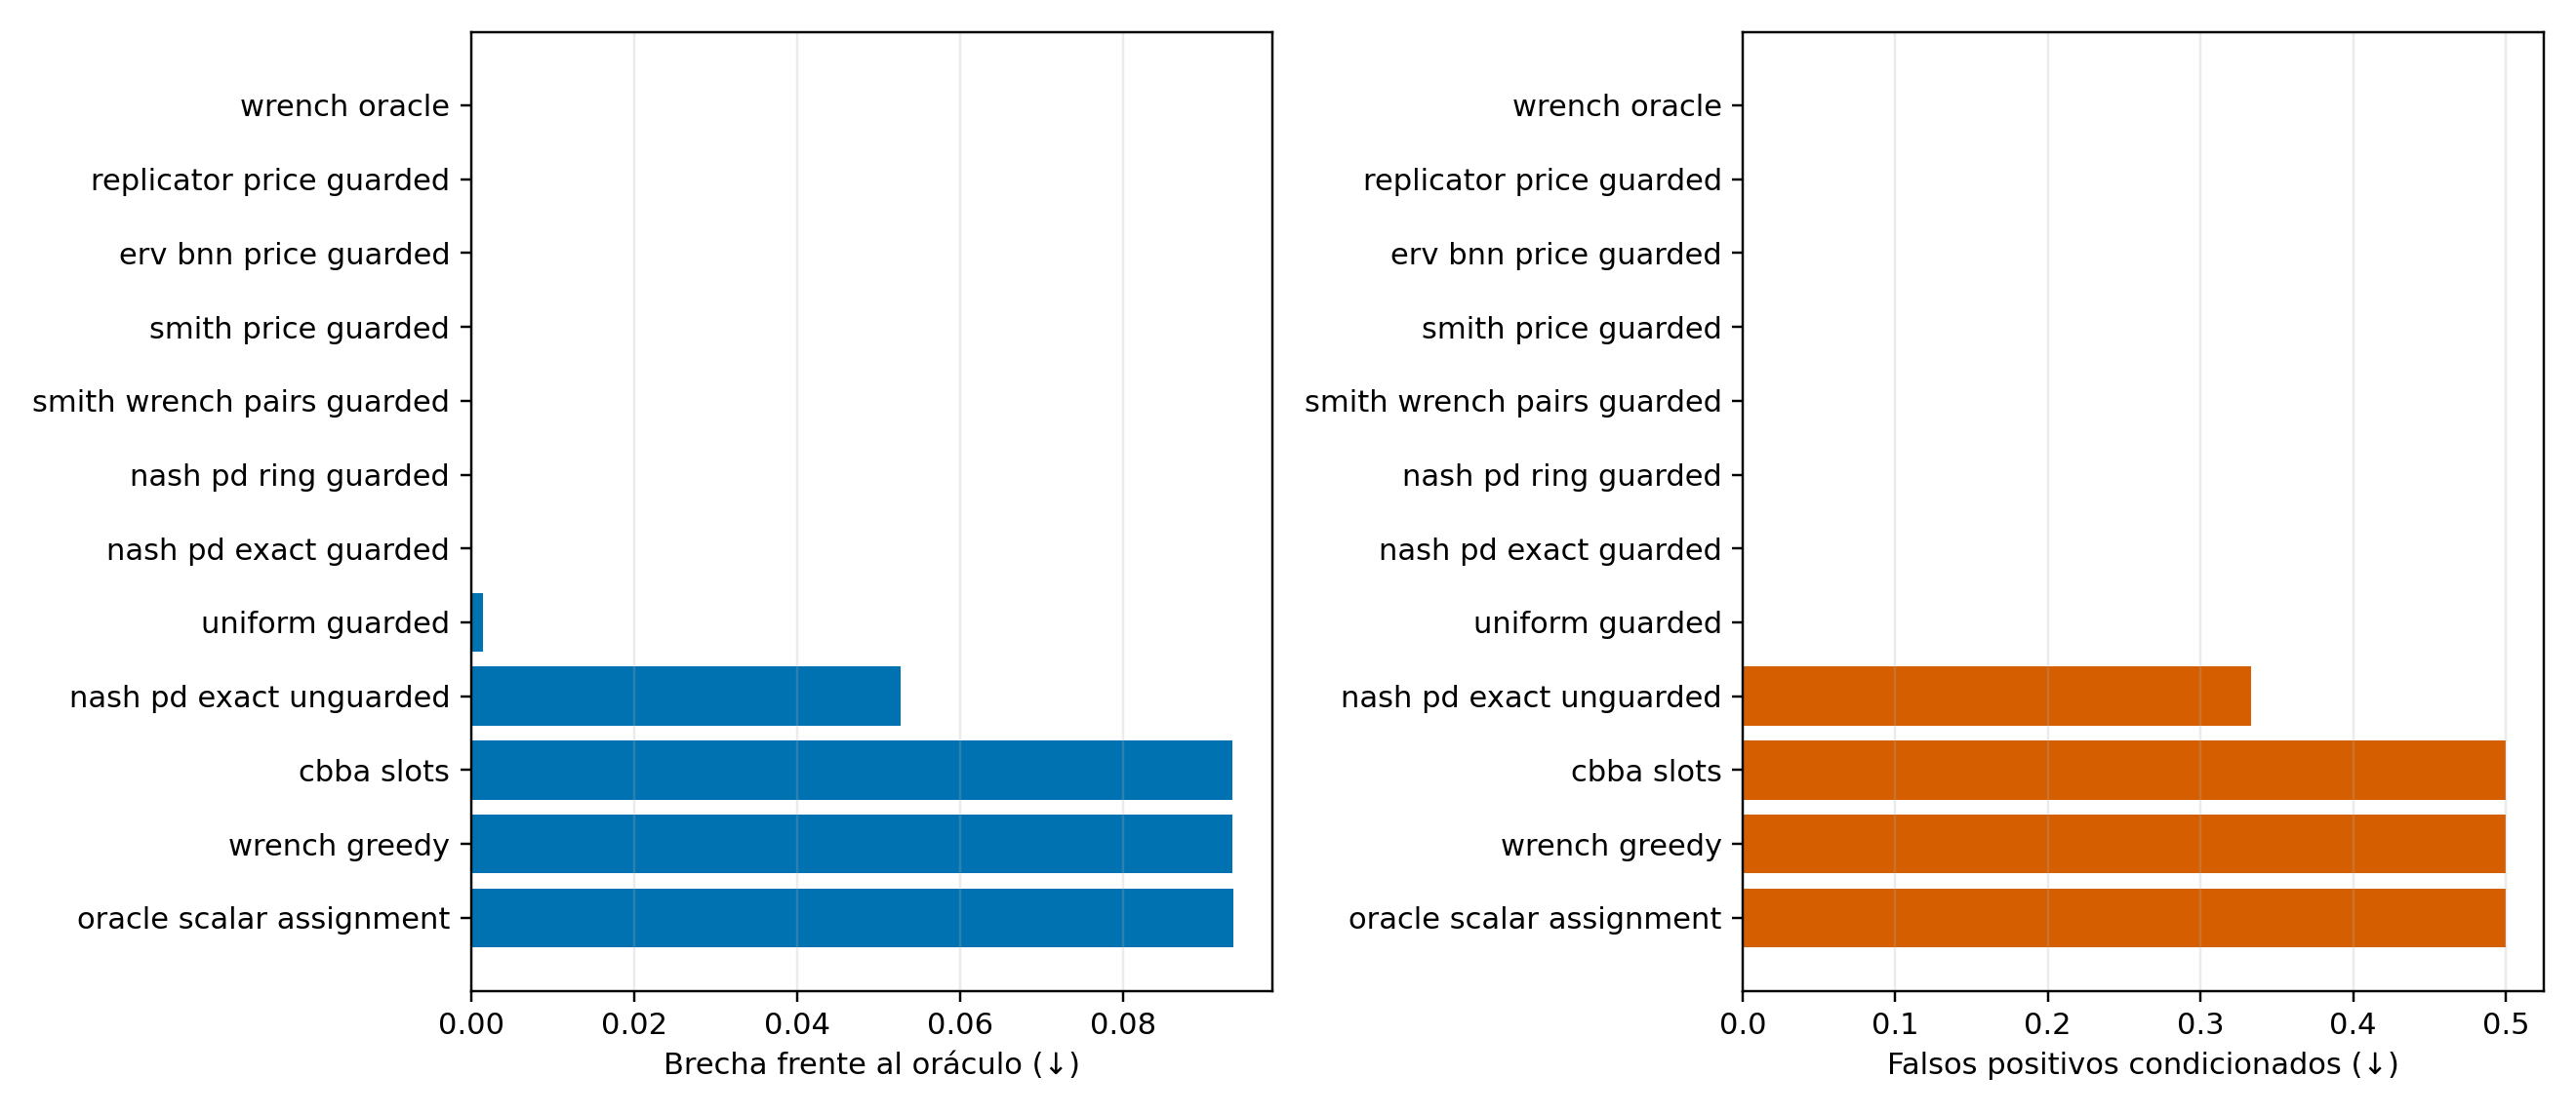
\includegraphics[width=0.92\textwidth]{figures/fig-sp3-wrench-game-performance.png}
\caption[Resultado decisivo de SP3]{Brecha respecto del oráculo y falsos positivos condicionados en SP3 v1.1.}
\viuownsource
\label{fig:sp3-wrench-game-performance}
\end{figure}

La lectura RAW vuelve a limitar la atribución. Uniforme+guardia también alcanzó cobertura completa y brecha $0{,}0015$; por tanto, el resultado CLOSED procede principalmente de la reparación global. SP3 respalda la formulación con restricciones compartidas, la equivalencia KKT/v-GNE de la relajación y la necesidad de comprobar el \emph{wrench}. No demuestra que el motor poblacional sea superior ni que el cierre sea distribuido de extremo a extremo.

\subsubsection{De la coalición a la misión: SP4--SP6}

\paragraph{SP4: juego de reclutamiento f\'isico hasta contactos seguros.}
\label{sec:resultados-sp4}

\medskip
\noindent\textbf{Frontera SP3--SP4--SP5.}
SP3 entrega una pose de contacto fija $g_i=(p_i^\star,\theta_i^\star)$ y una
prioridad wrench $\varpi_i$ para cada robot seleccionado. SP4 no vuelve a decidir
la coalici\'on ni transporta la carga: coordina el movimiento de los robots libres
hasta esas poses. SP5 comienza s\'olo despu\'es de que los robots est\'an acoplados y
la carga pasa a ser un cuerpo extendido m\'ovil. Esta frontera evita atribuir a la
planificaci\'on de SP4 la factibilidad wrench demostrada en SP3 o la estabilidad de
transporte estudiada en SP5.

El estado del robot diferencial es
$z_i=[p_{x,i},p_{y,i},\theta_i,v_i,\omega_i]^\top$ y evoluciona como
\begin{equation}
 \dot p_i=v_i[\cos\theta_i,\sin\theta_i]^\top,\qquad
 \dot\theta_i=\omega_i,\qquad
 \dot v_i=a_i,\qquad
 \dot\omega_i=\alpha_i .
 \label{eq:sp4-unicycle}
\end{equation}
Para masa $m_i$, inercia $J_i$, radio de rueda $r_w$ y v\'ia $b$, las fuerzas
longitudinales deseadas se transforman en pares
\begin{equation}
 \tau_{R,i}=r_w\left(\frac{m_i a_i}{2}+\frac{J_i\alpha_i}{b}\right),
 \qquad
 \tau_{L,i}=r_w\left(\frac{m_i a_i}{2}-\frac{J_i\alpha_i}{b}\right).
 \label{eq:sp4-wheel-torque}
\end{equation}
La simulaci\'on satura $\tau_R,\tau_L$, reconstruye $a_i,\alpha_i$ ejecutados e
integra \eqref{eq:sp4-unicycle} con paso $0{,}16$ s. No corrige posiciones despu\'es
de integrar. Un robot queda acoplado cuando, simult\'aneamente,
\begin{equation}
 \norm{p_i-p_i^\star}\leq0{,}18\ {\rm m},\quad
 |\operatorname{wrap}(\theta_i-\theta_i^\star)|\leq0{,}24\ {\rm rad},\quad
 |v_i|\leq0{,}16\ {\rm m\,s^{-1}}.
 \label{eq:sp4-docking}
\end{equation}
El \'exito seguro exige que todos los robots cumplan \eqref{eq:sp4-docking} antes
de 35 s y que el monitor barrido no detecte colisi\'on robot--robot,
robot--obst\'aculo, robot--carga ni frontera.

\begin{figure}[tbp]
\centering
\begin{tikzpicture}[
  node distance=6mm and 7mm,
  box/.style={draw=VIULinkBlue, rounded corners=1.5mm, fill=VIULight,
    minimum width=28mm, minimum height=12mm, align=center, font=\small},
  phys/.style={box, draw=VIUOrange, fill=VIUOrange!10},
  guard/.style={box, draw=VIUDeep, fill=VIUDeep!8},
  flow/.style={->, >=stealth, thick, draw=VIUDeep}
]
\node[phys] (sp3) {SP3\\contactos y\\prioridad wrench};
\node[box, right=of sp3] (primitives) {Seis primitivas\\espacio--tiempo};
\node[box, right=of primitives] (game) {Juego potencial\\PD / Smith /\\replicator / BNN};
\node[box, right=of game] (fractional) {Preferencia\\$x_i\in\Delta^6$};

\node[guard, below=of fractional] (closure) {Cierre discreto\\sin conflicto};
\node[box, left=of closure] (raw) {RAW\\$(v_i^d,\omega_i^d)$};
\node[guard, left=of raw] (safe) {SAFE\\proyeccion CBF};
\node[phys, left=of safe] (plant) {EXEC\\par de ruedas\\y uniciclo};

\node[guard, below=of plant] (monitor) {Monitor barrido\\sin reparacion};
\node[phys, right=of monitor] (dock) {Pose de contacto\\y velocidad nula};
\node[phys, right=of dock] (sp5) {SP5\\transporte de\\carga acoplada};

\draw[flow] (sp3) -- (primitives);
\draw[flow] (primitives) -- (game);
\draw[flow] (game) -- (fractional);
\draw[flow] (fractional) -- (closure);
\draw[flow] (closure) -- (raw);
\draw[flow] (raw) -- (safe);
\draw[flow] (safe) -- (plant);
\draw[flow] (plant) -- (monitor);
\draw[flow] (monitor) -- (dock);
\draw[flow] (dock) -- (sp5);
\draw[flow, dashed] (monitor.east) to[bend right=18]
  node[below, font=\scriptsize, align=center]{estado ejecutado\\y precios} (primitives.south);
\end{tikzpicture}
\caption[Arquitectura RAW--SAFE--EXEC de SP4]{SP4 recibe de SP3 contactos fijos y prioridad wrench, coordina clases de ruta mediante un juego de primitivas, filtra seguridad antes de ejecutar una planta no holonoma saturada y entrega a SP5 robots acoplados.}
\viuownsource
\label{fig:sp4-docking-game-architecture}
\end{figure}

\medskip
\noindent\textbf{Juego de primitivas espacio--tiempo.}
En cada replanteo, el robot $i$ distribuye una preferencia
$x_i\in\Delta^6$ sobre cinco primitivas de movimiento y una de espera. Las
primitivas representan dos arcos horarios, la ruta angular localmente corta, dos
arcos antihorarios y espera/alineaci\'on. Si la carga separa al robot de su contacto,
la clase horaria o antihoraria elegida se conserva hasta que el segmento directo
sea geom\'etricamente libre. La memoria de homotop\'ia impide cambios inducidos
por el horizonte recedente; no constituye un plan global.

Sea $H_{ia,r}\in\{0,1\}$ la ocupaci\'on de la celda espacio--tiempo $r$ por la
acci\'on $a$ del robot $i$ en los tiempos de predicci\'on
$0{,}45$, $0{,}90$, $1{,}35$ y $1{,}80$ s. El coste congelado $c_{ia}$ combina
distancia terminal ponderada por $\varpi_i$, error angular, esfuerzo, proximidad
a obst\'aculos, espera y cambio de clase de ruta. La relajaci\'on minimiza
\begin{equation}
 \Phi(x)=
 \sum_{i,a}c_{ia}x_{ia}
 +\frac{\beta}{2}\left\|\sum_i H_i x_i\right\|_2^2
 +\frac{\epsilon}{2}\sum_i\norm{x_i}_2^2,
 \qquad
 \sum_i H_i x_i\leq\mathbf 1 ,
 \label{eq:sp4-potential}
\end{equation}
con $\beta=0{,}38$ y $\epsilon=0{,}04$. La construcci\'on sigue la idea de usar
un potencial com\'un para coordinar decisiones locales
\citep{monderer1996potential,hurtado2024potential}, pero aqu\'i las acciones son
primitivas no hol\'onomas y los recursos son celdas espacio--tiempo.

\begin{proposicion}[Potencial exacto de la instant\'anea]
Para una instant\'anea con $c$ y $H$ fijos, el pseudogradiente del juego coincide
por bloques con $\nabla\Phi$. Por tanto, toda desviaci\'on unilateral cambia el
coste del jugador en la misma direcci\'on que el potencial.
\end{proposicion}
\begin{proof}
Si $y=\sum_jH_jx_j$, entonces
\[
 \nabla_{x_i}\Phi=c_i+\beta H_i^\top y+\epsilon x_i.
\]
La parte que depende de $x_i$ en el coste del jugador puede escribirse como
$c_i^\top x_i+\frac{\beta}{2}\norm{H_ix_i}^2+
\beta(H_ix_i)^\top\sum_{j\neq i}H_jx_j+
\frac{\epsilon}{2}\norm{x_i}^2$. Su gradiente es la expresi\'on anterior.
Integrar el gradiente a lo largo de una desviaci\'on unilateral prueba la
identidad de potencial.
\end{proof}

Con un multiplicador compartido $\lambda\geq0$, las KKT de la relajaci\'on son
\begin{equation}
\begin{aligned}
 0&\in c_i+\beta H_i^\top Hx+\epsilon x_i+H_i^\top\lambda
       +N_{\Delta^6}(x_i),\\
 0&\leq\lambda\perp\mathbf1-Hx\geq0 .
\end{aligned}
\label{eq:sp4-kkt}
\end{equation}
Si existe Slater, la convexidad de \eqref{eq:sp4-potential} hace estas condiciones
necesarias y suficientes para el \'optimo de la instant\'anea; al compartir
$\lambda$, ese punto es el v-GNE de la relajaci\'on. La caracterizaci\'on variacional
mediante un multiplicador compartido para restricciones acopladas sigue el marco de
\citet{yi2019operator}. La convergencia de din\'amicas primal--dual restringidas
requiere las hip\'otesis de regularidad estudiadas por
\citet{cherukuri2016primaldual}. Estas referencias no prueban optimalidad de la
trayectoria no lineal completa.

El protocolo Nash--PD aplica
\begin{equation}
 x_i^{+}=\Pi_{\Delta^6}\!\left[
 x_i-\eta\left(c_i+\beta H_i^\top\widehat y_i+\epsilon x_i+
 H_i^\top\lambda_i\right)\right],\qquad
 \lambda_i^{+}=\left[\lambda_i+\eta_\lambda(\widehat y_i-\mathbf1)\right]_+ .
 \label{eq:sp4-pd}
\end{equation}
La variante exacta usa el agregado $y=Hx$; la variante en anillo ejecuta cuatro
rondas Metropolis por iteraci\'on. Como ablaci\'on del motor, el mismo payoff
negativo alimenta Smith, replicator y ERV--BNN. Replicator y BNN siguen
\begin{equation}
 \dot x_{ia}^{\rm rep}=x_{ia}(\pi_{ia}-\bar\pi_i),\qquad
 \dot x_{ia}^{\rm BNN}=[\pi_{ia}-\bar\pi_i]_+
 -x_{ia}\sum_b[\pi_{ib}-\bar\pi_i]_+ .
 \label{eq:sp4-population}
\end{equation}
La proyecci\'on num\'erica conserva el s\'implex en los cuatro protocolos. El teorema
KKT se aplica al projected primal--dual con informaci\'on exacta bajo sus
hip\'otesis; no se transfiere autom\'aticamente a Smith, replicator, BNN ni a consenso
finito.

Para $A=6$ acciones y $R$ recursos, evaluar gradiente y ocupaci\'on cuesta
$O(NAR)$ por iteraci\'on; Smith a\~nade comparaciones $O(NA^2)$ y el consenso cuesta
$O(L|E|R)$ para $L$ rondas. El QP convexo de una instant\'anea es polinomial con
datos racionales, pero el cierre entero de rutas con conflictos contiene
\emph{set packing} y es NP-hard en general. La campa\~na implementa un cierre
\emph{greedy}, no un solver entero \'optimo.

\medskip
\noindent\textbf{Cierre, barrera y separaci\'on RAW--SAFE--EXEC.}
RAW selecciona el \emph{argmax} de cada preferencia. La variante cerrada ordena
robots por prioridad wrench y elige para cada uno la primitiva mejor valorada que
no reutiliza un recurso ya reservado. Este cierre observa todas las preferencias
y recursos; por tanto, es un postproceso global y no acredita distribuci\'on
extremo a extremo. La ablaci\'on Nash--PD RAW permite medir su efecto.

La seguridad se impone sobre el punto adelantado
$y_i=p_i+\ell[\cos\theta_i,\sin\theta_i]^\top$, con $\ell=0{,}02$ m. Para dos
robots se usa
\begin{equation}
 h_{ij}=\norm{y_i-y_j}^2-d_{ij}^2,\qquad
 2(y_i-y_j)^\top(\dot y_i-\dot y_j)+\gamma h_{ij}\geq0 ,
 \label{eq:sp4-cbf-pair}
\end{equation}
donde $d_{ij}=2r_{\rm rob}+m_s+2|\ell|$. Para un obst\'aculo circular, el radio
se infla en $r_{\rm rob}+m_s+|\ell|$. Estas inflaciones usan la desigualdad
triangular para que separar los puntos adelantados implique separar los discos.
La velocidad SAFE se obtiene por proyecciones alternadas sobre los semiespacios
de \eqref{eq:sp4-cbf-pair}, con cotas de aceleraci\'on alcanzable. Es una
proyecci\'on CBF, no un QP monol\'itico. Las CBF formalizan invariancia hacia
adelante para el modelo y las hip\'otesis declaradas \citep{ames2017cbf}.

EXEC transforma SAFE a pares de rueda, satura e integra la planta. Como la
saturaci\'on puede romper una desigualdad cinem\'atica, el residual CBF se vuelve a
evaluar con la velocidad ejecutada y la colisi\'on se determina mediante distancia
m\'inima entre segmentos consecutivos. No hay teleportaci\'on, separaci\'on
geom\'etrica posterior ni reparaci\'on de una trayectoria ya ejecutada.

\medskip
\noindent\textbf{Dise\~no confirmatorio.}
El piloto v2 se us\'o s\'olo para comprobar factibilidad y congelar el protocolo.
La campa\~na confirmatoria abre semillas nuevas y cruza seis escenarios
abierto, cruce, pasaje estrecho, obst\'aculos dispersos, bloqueo sim\'etrico y
actuadores limitados, con $N\in\{4,8,12\}$. Se comparan movimiento directo,
APF, un proxy RVO, proyecci\'on CBF, PD central con 70 iteraciones, Nash--PD RAW,
Nash--PD exacto y en anillo, Smith, replicator y ERV--BNN. Los mundos son
id\'enticos entre m\'etodos.

Las m\'etricas primarias son \'exito seguro y cualquier colisi\'on barrida. Se
a\~naden tiempo truncado, error final, despeje, energ\'ia de rueda, saturaciones,
intervenci\'on de barrera, residual KKT, mensajes y tiempo de c\'omputo. Cinco
contrastes se congelaron antes de abrir la confirmatoria: \'exito de replicator
frente a CBF; colisi\'on de replicator frente a directo; KKT exacto frente a
anillo; \'exito de replicator frente a Nash--PD; y error posicional de replicator
frente a PD central. Las tasas usan prueba binomial exacta sobre pares discordantes;
las variables continuas usan Wilcoxon unilateral. Se informa bootstrap pareado del
95\,\% y correcci\'on de Holm.
La unidad de aleatorizaci\'on no es cada fila de escenario: las seis variantes
comparten la semilla dentro de cada pareja $(\texttt{seed},N)$, por lo que la
confirmatoria contiene 18 bloques independientes y 108 filas emparejadas. Las
tasas y los intervalos anteriores se conservan como descripci\'on por escenario;
como sensibilidad inferencial se agreg\'o primero por bloque y se aplic\'o una
prueba de signos unilateral con Holm. Los cinco contrastes mantuvieron el signo
y el rechazo a $\alpha=0{,}05$ (p ajustadas $0{,}0352$, $1{,}91\times10^{-5}$,
$1{,}45\times10^{-4}$, $1{,}91\times10^{-5}$ y $1{,}91\times10^{-5}$,
ordenadas por hip\'otesis). En consecuencia no se interpreta el total de 108
filas como 108 observaciones IID.

\medskip
\noindent\textbf{Resultados confirmatorios.}
La candidata can\'onica \texttt{SP4\_DOCKING\_GAME\_CONFIRMATORY\_v3} contiene
18 bloques independientes, 108 instancias pareadas y 1188 ejecuciones: seis semillas nuevas, seis escenarios, tres
tama\~nos de flota y once m\'etodos. La auditor\'ia termin\'o en PASS. No hubo
colisiones iniciales; el despeje inicial m\'inimo fue $0{,}2724$ m. El error
m\'aximo del s\'implex fue $2{,}22\times10^{-16}$, la violaci\'on de capacidad fue
cero, la brecha m\'axima frente al QP independiente fue $1{,}139\times10^{-4}$ y
el error de gradiente fue $8{,}07\times10^{-10}$. Los seis QP auditados
convergieron y no se repar\'o ninguna posici\'on.

\begin{table}[tbp]
\centering
\caption{Resultados confirmatorios de SP4 v3. KKT no aplica a los comparadores sin juego.}
\label{tab:sp4-v3-main}
\scriptsize
\begin{tabular}{@{}lrrrrr@{}}
\toprule
M\'etodo & \'Exito & Colisi\'on & Timeout & KKT & Tiempo (s)\\
\midrule
Directo al contacto & 0,1667 & 0,8333 & 0,0000 & -- & 0,025\\
APF & 0,1111 & 0,7593 & 0,1296 & -- & 0,136\\
RVO proxy & 0,1667 & 0,8333 & 0,0000 & -- & 0,028\\
Proyecci\'on CBF & 0,1759 & 0,0000 & 0,8241 & -- & 1,598\\
PD central (70 iter.) & 0,0370 & 0,0000 & 0,9630 & 0,0661 & 2,939\\
Nash--PD RAW & 0,0278 & 0,0000 & 0,9722 & 0,0576 & 1,843\\
Nash--PD exacto & 0,0278 & 0,0000 & 0,9722 & 0,0892 & 1,767\\
Nash--PD anillo & 0,0093 & 0,0000 & 0,9907 & 0,4244 & 2,038\\
Smith + CBF & 0,0093 & 0,0000 & 0,9907 & 0,1286 & 2,164\\
Replicator + CBF & 0,2685 & 0,0000 & 0,7315 & 1,7036 & 2,250\\
ERV--BNN + CBF & 0,0000 & 0,0000 & 1,0000 & 0,1884 & 2,157\\
\bottomrule
\end{tabular}
\end{table}

Replicator obtuvo la mayor tasa de \'exito seguro, $0{,}2685$ (IC95\,\%
$[0{,}1852,0{,}3519]$), frente a $0{,}1759$ de la proyecci\'on CBF y
$0{,}0278$ de Nash--PD exacto. Esta ventaja no equivale a completitud:
$0{,}7315$ de sus mundos terminaron por tiempo. Los m\'etodos guardados no
colisionaron; directo y RVO colisionaron en $0{,}8333$ y APF en $0{,}7593$.
Por tanto, la llegada de los controles directos no es un \'exito seguro.

\begin{figure}[tbp]
\centering
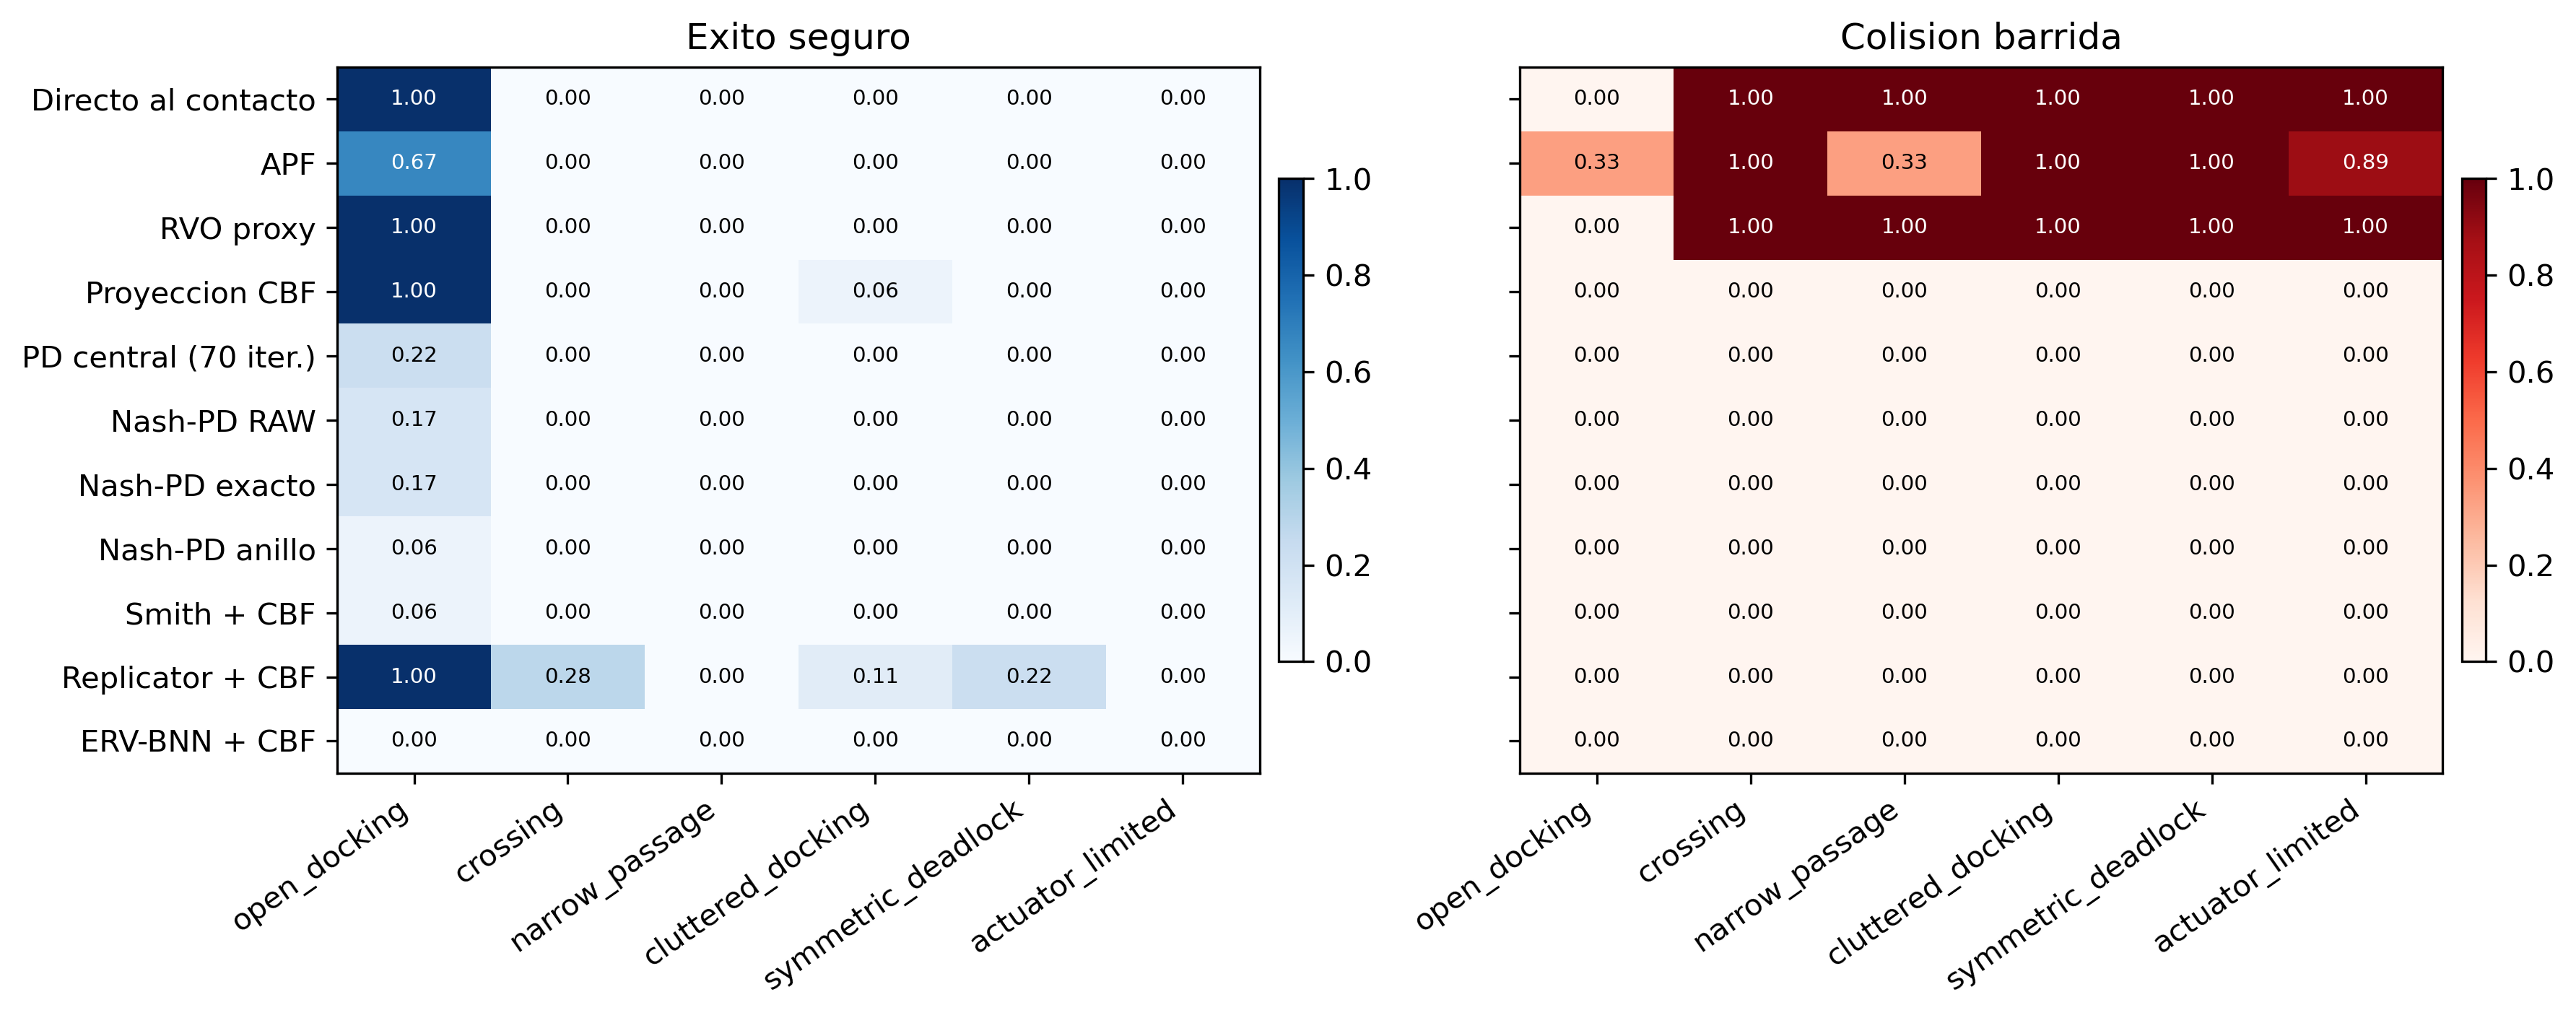
\includegraphics[width=\textwidth]{figures/fig-sp4-scenario-matrix.png}
\caption[\'Exito y colisi\'on por escenario en SP4]{Matriz confirmatoria por
m\'etodo y escenario. Replicator resuelve parte de cruce, bloqueo sim\'etrico y
obst\'aculos dispersos, pero no el pasaje estrecho ni los actuadores limitados.}
\viuownsource
\label{fig:sp4-scenario-matrix}
\end{figure}

La estratificaci\'on impide convertir el promedio en una afirmaci\'on general.
Replicator alcanz\'o $1{,}000$ en abierto, $0{,}278$ en cruce, $0{,}222$ en
bloqueo sim\'etrico y $0{,}111$ con obst\'aculos dispersos; obtuvo cero en pasaje
estrecho y actuadores limitados. La proyecci\'on CBF alcanz\'o $1{,}000$ en
abierto y $0{,}056$ con obst\'aculos dispersos, pero cero en los otros cuatro
escenarios.

A nivel descriptivo de las 108 instancias, Replicator aument\'o el éxito frente a
CBF en $0{,}0926$ (IC95\,\% $[0{,}0370,0{,}1574]$) y frente a Nash--PD en
$0{,}2407$ ($[0{,}1574,0{,}3241]$); redujo la colisión frente a directo en
$0{,}8333$ ($[-0{,}8981,-0{,}7593]$), y el error posicional frente a PD central
en $1{,}0436$~m ($[-1{,}1881,-0{,}9067]$). La información exacta redujo el
residual KKT frente al anillo en $0{,}3351$ ($[-0{,}3952,-0{,}2760]$). Esos
intervalos describen instancias; no se usan como si los seis escenarios dentro de
semilla--flota fueran independientes.

\begin{table}[tbp]
\centering
\scriptsize
\begin{tabularx}{\textwidth}{@{}Xrrrr@{}}
\toprule
Hipótesis (dirección favorable) & Bloques $+/-/=$ & Diferencia media original & $p$ exacta & $p_{\rm Holm}$ \\
\midrule
H4.1: éxito Replicator $>$ CBF & 7/1/10 & $0{,}0926$ & $0{,}0352$ & $0{,}0352$ \\
H4.2: colisión Replicator $<$ directo & 18/0/0 & $-0{,}8333$ & $3{,}81\times10^{-6}$ & $1{,}91\times10^{-5}$ \\
H4.3: KKT exacto $<$ anillo & 17/1/0 & $-0{,}3351$ & $7{,}25\times10^{-5}$ & $1{,}45\times10^{-4}$ \\
H4.4: éxito Replicator $>$ Nash--PD & 18/0/0 & $0{,}2407$ & $3{,}81\times10^{-6}$ & $1{,}91\times10^{-5}$ \\
H4.5: error Replicator $<$ PD central & 18/0/0 & $-1{,}0436$ & $3{,}81\times10^{-6}$ & $1{,}91\times10^{-5}$ \\
\bottomrule
\end{tabularx}
\caption{Sensibilidad inferencial de SP4 sobre 18 bloques independientes. El signo se orienta según la dirección preespecificada; los empates se excluyen del test de signos exacto.}
\label{tab:sp4-block-sensitivity}
\end{table}

\begin{figure}[tbp]
\centering
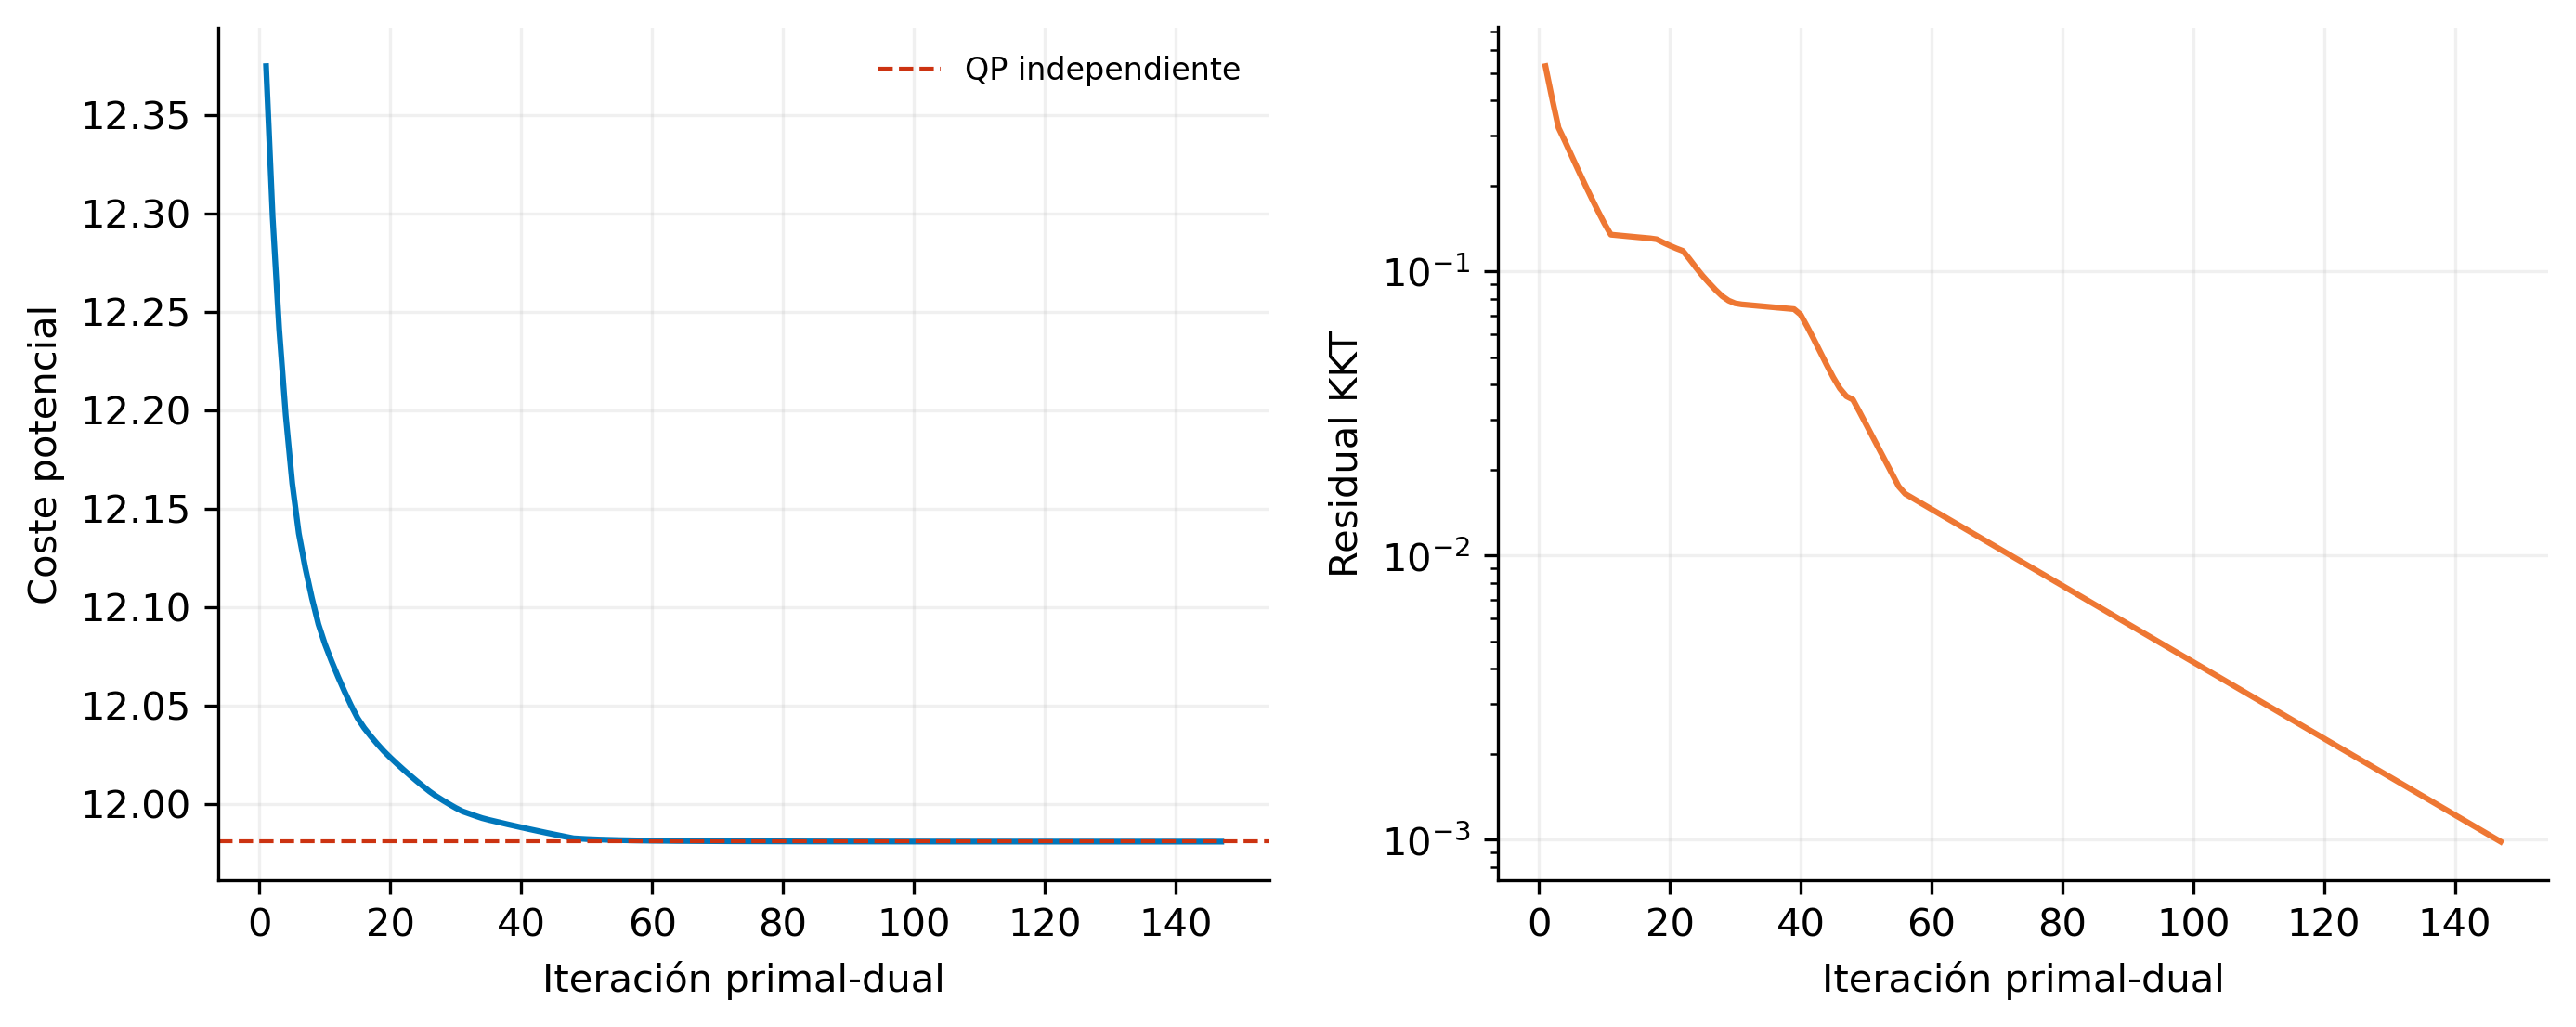
\includegraphics[width=0.86\textwidth]{figures/fig-sp4-kkt-potential.png}
\caption[Auditor\'ia del potencial de SP4]{Evoluci\'on del coste y residual KKT
de una instant\'anea auditada frente al QP convexo independiente.}
\viuownsource
\label{fig:sp4-kkt-potential}
\end{figure}

La disminuci\'on de KKT no predijo el \'exito cerrado. Replicator obtuvo residual
medio $1{,}7036$, pero la mayor llegada; Nash--PD exacto redujo KKT a $0{,}0892$
y casi siempre agot\'o el horizonte. Esto sugiere que el transitorio de revisi\'on
y la secuencia de primitivas importan m\'as que resolver con precisi\'on cada
instant\'anea miope. Adem\'as, Nash--PD RAW y cerrado empataron en \'exito
($0{,}0278$): las $6{,}26$ intervenciones medias del cierre no explican una
mejora terminal en esta campa\~na.

\begin{figure}[tbp]
\centering
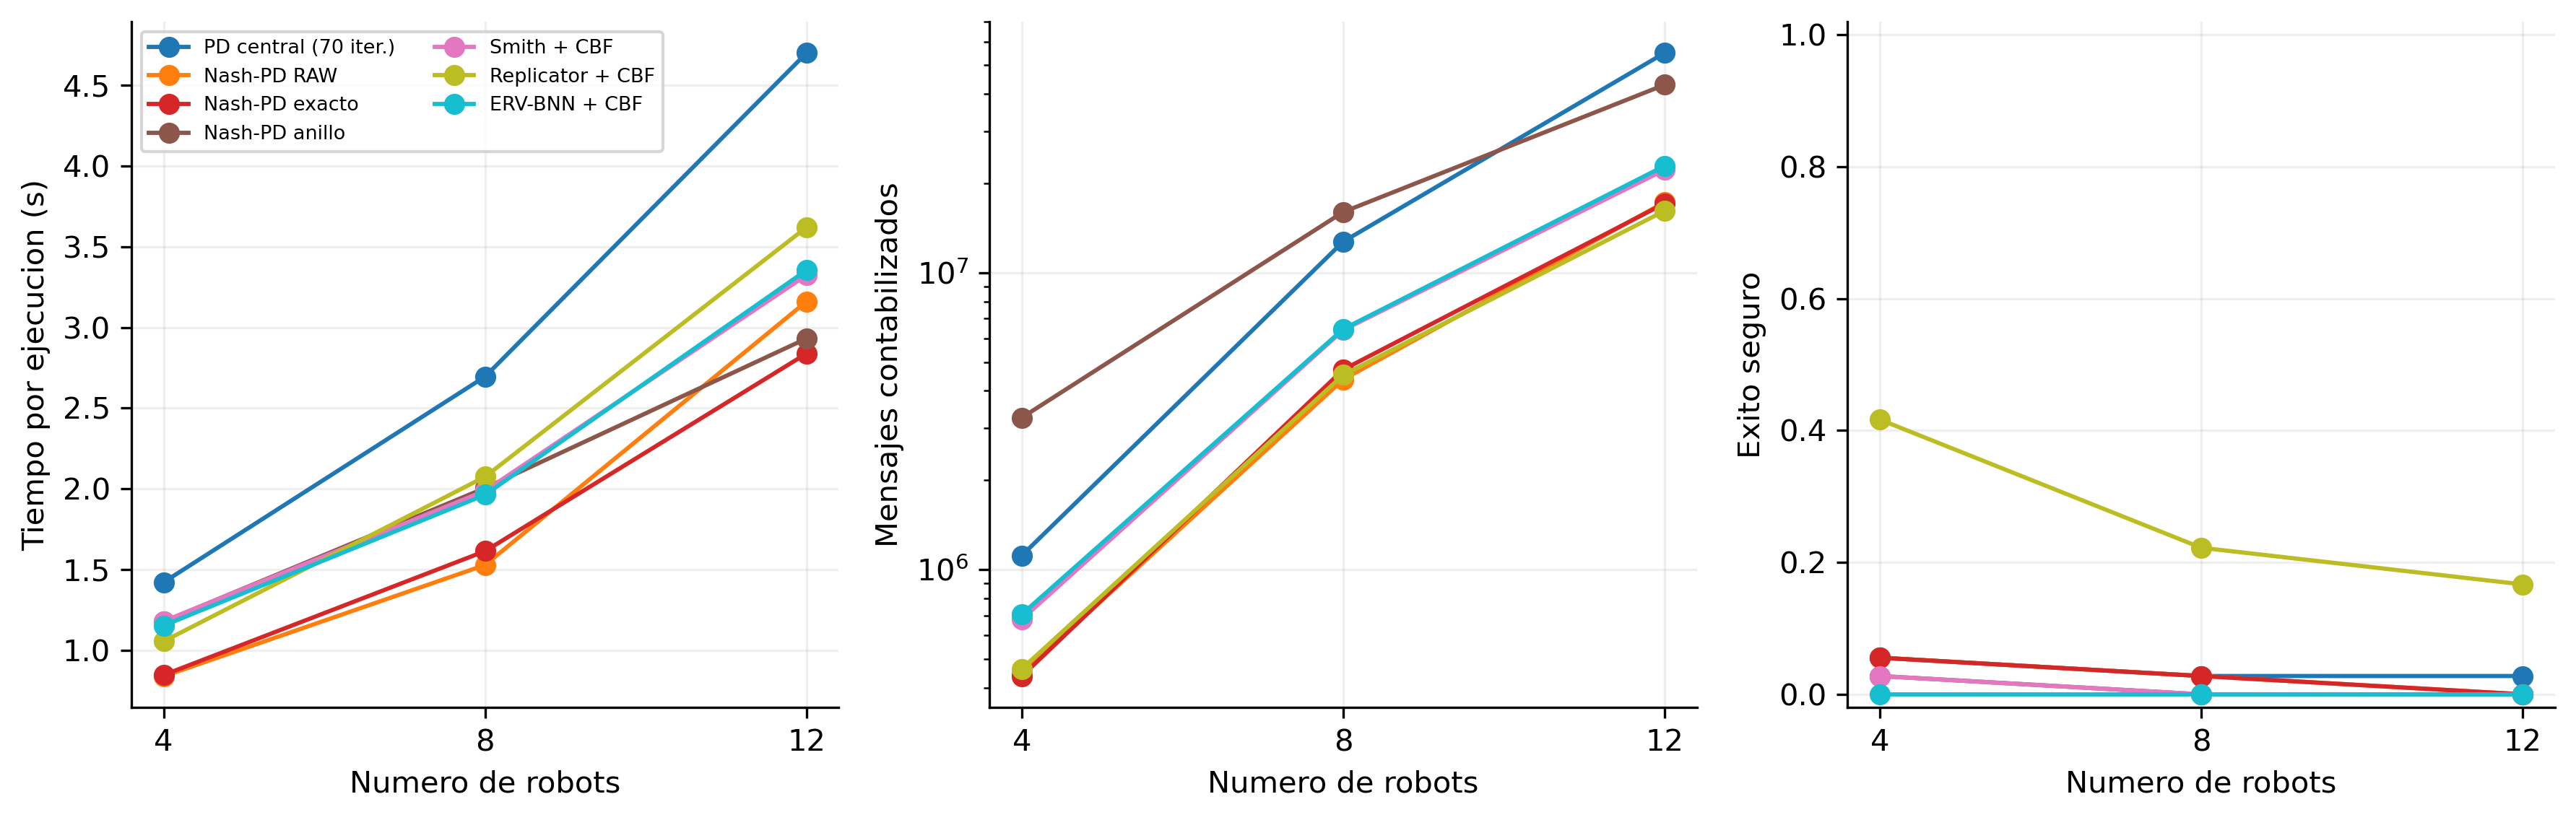
\includegraphics[width=\textwidth]{figures/fig-sp4-scaling.png}
\caption[Escalado observado de SP4]{Tiempo, mensajes contabilizados y \'exito
seguro para los m\'etodos de juego al pasar de 4 a 12 robots.}
\viuownsource
\label{fig:sp4-scaling}
\end{figure}

El \'exito de replicator cay\'o de $0{,}4167$ con cuatro robots a $0{,}2222$ con
ocho y $0{,}1667$ con doce. Su tiempo subi\'o de $1{,}06$ a $3{,}62$ s y los
mensajes contabilizados de $4{,}62\times10^5$ a $1{,}62\times10^7$. En el
anillo, los mensajes alcanzaron $4{,}30\times10^7$ con doce robots. Son medidas
del simulador, no cotas asint\'oticas ni latencia de red real.

Finalmente, no hubo saturaciones de par en las 1188 ejecuciones. La campa\~na
modela la transformaci\'on y los l\'imites, pero no excita esa no linealidad y no
valida robustez frente a saturaci\'on. Tambi\'en aparecieron residuales CBF EXEC
positivos: $48{,}64$ pasos por ejecuci\'on en replicator y $98{,}81$ en CBF,
en promedio, aunque el monitor barrido no registr\'o colisiones. Por ello, el
cero emp\'irico de colisi\'on no demuestra seguridad continua despu\'es
de la ejecuci\'on.

\medskip
\noindent\textbf{Alcance.}
La contribuci\'on de SP4 es la formulaci\'on y auditor\'ia de un juego recedente
wrench-aware sobre una planta no hol\'onoma saturada, no una demostraci\'on de
optimalidad global. La equivalencia QP/KKT se limita a instant\'aneas convexas; la
composici\'on con cierre, replanteo, CBF y pares saturados se eval\'ua
experimentalmente. El cierre y la informaci\'on completa siguen siendo globales.
El proxy RVO no es una implementaci\'on completa de ORCA. La carga permanece fija:
la estabilidad del transporte y la fricci\'on de contacto son preguntas de SP5 y
de validaci\'on f\'isica futura.


\paragraph{SP5: transporte de la carga como cuerpo extendido.}
SP5 v2 comienza donde termina SP4: los robots ya están acoplados a contactos
fijos de la carga. La planta integra
$M\ddot q+D\dot q=w_{\rm EXEC}+d$ y conserva por separado el \emph{wrench}
nominal (RAW), la orden filtrada (SAFE) y el \emph{wrench} realizable tras
límites individuales (EXEC). No se corrigen posiciones después de integrar.
El protocolo congeló seis escenarios, $N\in\{4,8,12\}$, seis semillas nuevas y
ocho métodos: 108 mundos emparejados y 864 ejecuciones exclusivamente CPU.

El CBF local alcanzó $0{,}593$ de éxito seguro sin colisiones. El proxy VO
alcanzó $0{,}657$, pero colisionó en $0{,}343$ de los mundos. La variante
Hamiltoniana RAW obtuvo $0{,}167$ de éxito y $0{,}833$ de colisión. Al añadir
CBF pasó a $0{,}426$ y cero colisiones. Las diferencias de colisión
$-0{,}833$ y éxito $0{,}259$ sobrevivieron Holm. El preview distribuido también
redujo la colisión frente a VO en $0{,}343$. En cambio, la referencia
centralizada fue conservadora: solo alcanzó $0{,}167$ y no superó al CBF local.
Tampoco se respald\'o la direcci\'on preespecificada del contraste CBF--APF sobre
residual EXEC: pese a $p_{\rm Holm}=0{,}0038$, el efecto medio fue $+0{,}0012$ y el IC95\% $[-0{,}0305,0{,}0390]$ incluy\'o cero, de modo que el rango pareado no autoriza una mejora en la direcci\'on exigida.

\begin{figure}[tbp]
\centering
\begin{minipage}[t]{0.49\textwidth}
\centering
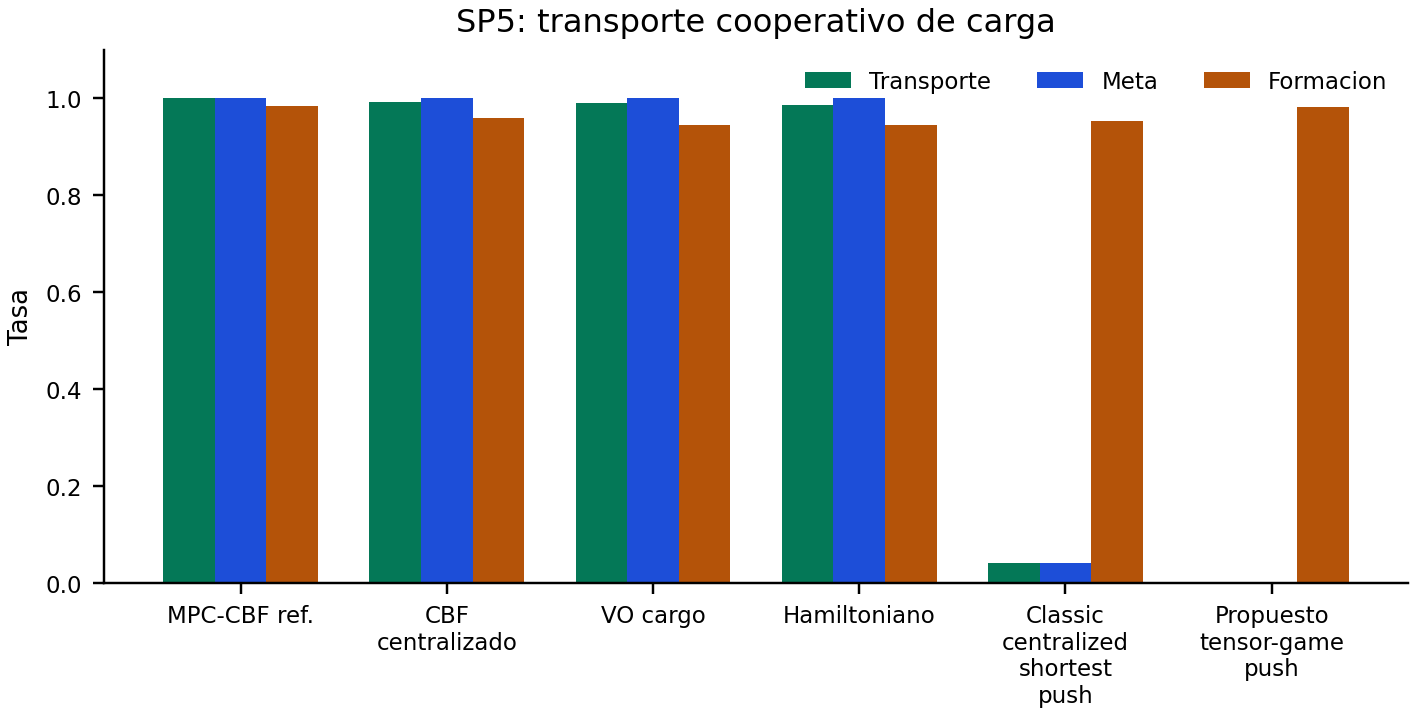
\includegraphics[width=\linewidth]{figures/fig-sp5-primary.png}
\end{minipage}\hfill
\begin{minipage}[t]{0.49\textwidth}
\centering
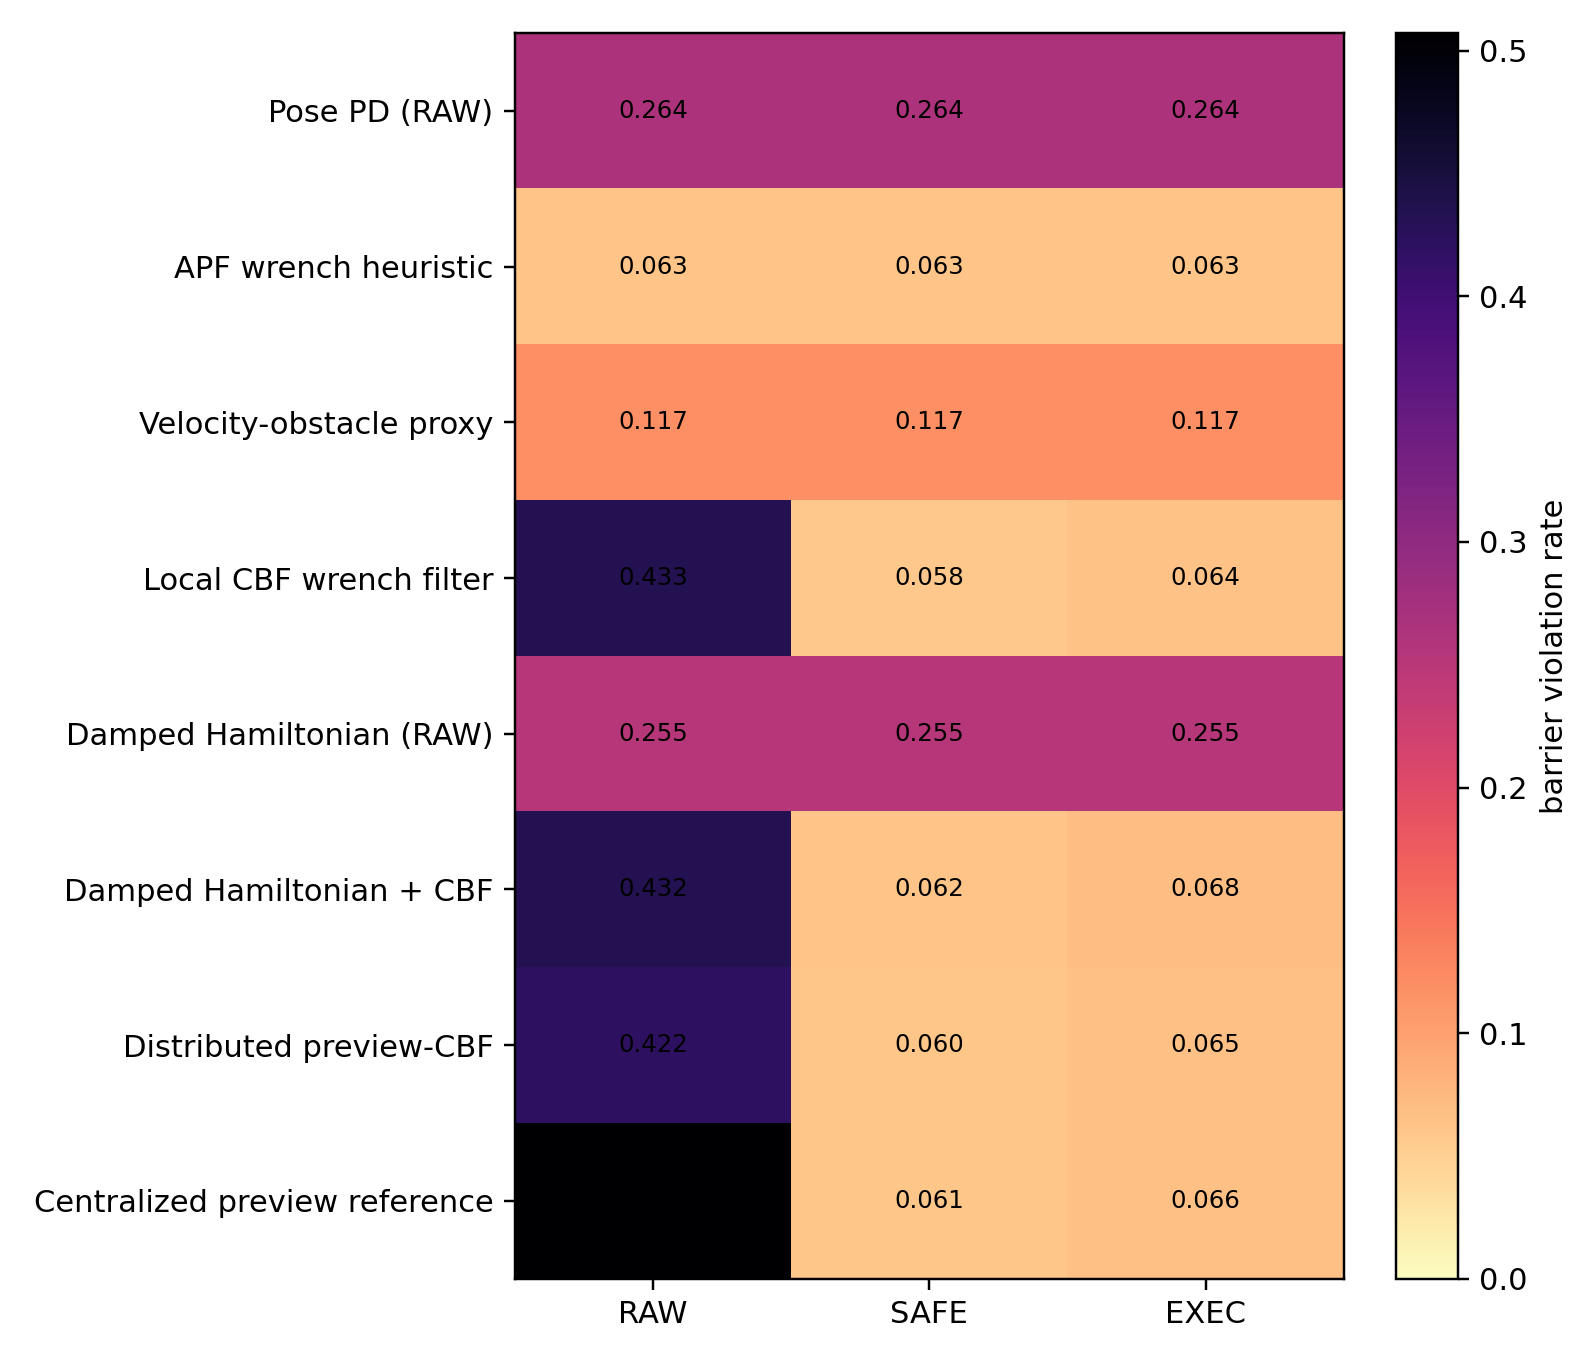
\includegraphics[width=\linewidth]{figures/fig-sp5-raw-safe-exec.png}
\end{minipage}
\caption[Resultado y ablación mecánica de SP5]{éxito/colisión por método
(izquierda) y residuo de barrera en RAW, SAFE y EXEC (derecha). La seguridad se
decide sobre la trayectoria ejecutada, no sobre la orden filtrada.}
\viuownsource
\label{fig:sp5-canonical-v2}
\end{figure}

El bloque histórico de 20.040 filas se conserva, pero dejó de ser canónico:
proyectaba carga y robots fuera de los obstáculos después de cada paso. SP5 v2
respalda la necesidad de separar seguridad comandada y mecánica ejecutada; no
demuestra contacto con fricción, dinámica de rueda, seguridad funcional ni
superioridad universal del controlador Hamiltoniano.

\paragraph{SP6: reparación después de eventos.}
SP6 elimina robots no disponibles, incorpora reemplazos y vuelve a comprobar el residual antes de declarar recuperación. En 20.000 ejecuciones, el mercado \emph{wrench} con guardia obtuvo completitud $0{,}7117$, recuperación $0{,}5155$ y factibilidad posterior al evento $0{,}9673$. La pérdida de carga disminuyó en $0{,}0227$ frente a \emph{greedy} ($p_{\rm Holm}<0{,}001$). La diferencia de completitud frente a Smith-QR fue $0{,}0044$ y no resultó concluyente.

\begin{figure}[tbp]
\centering
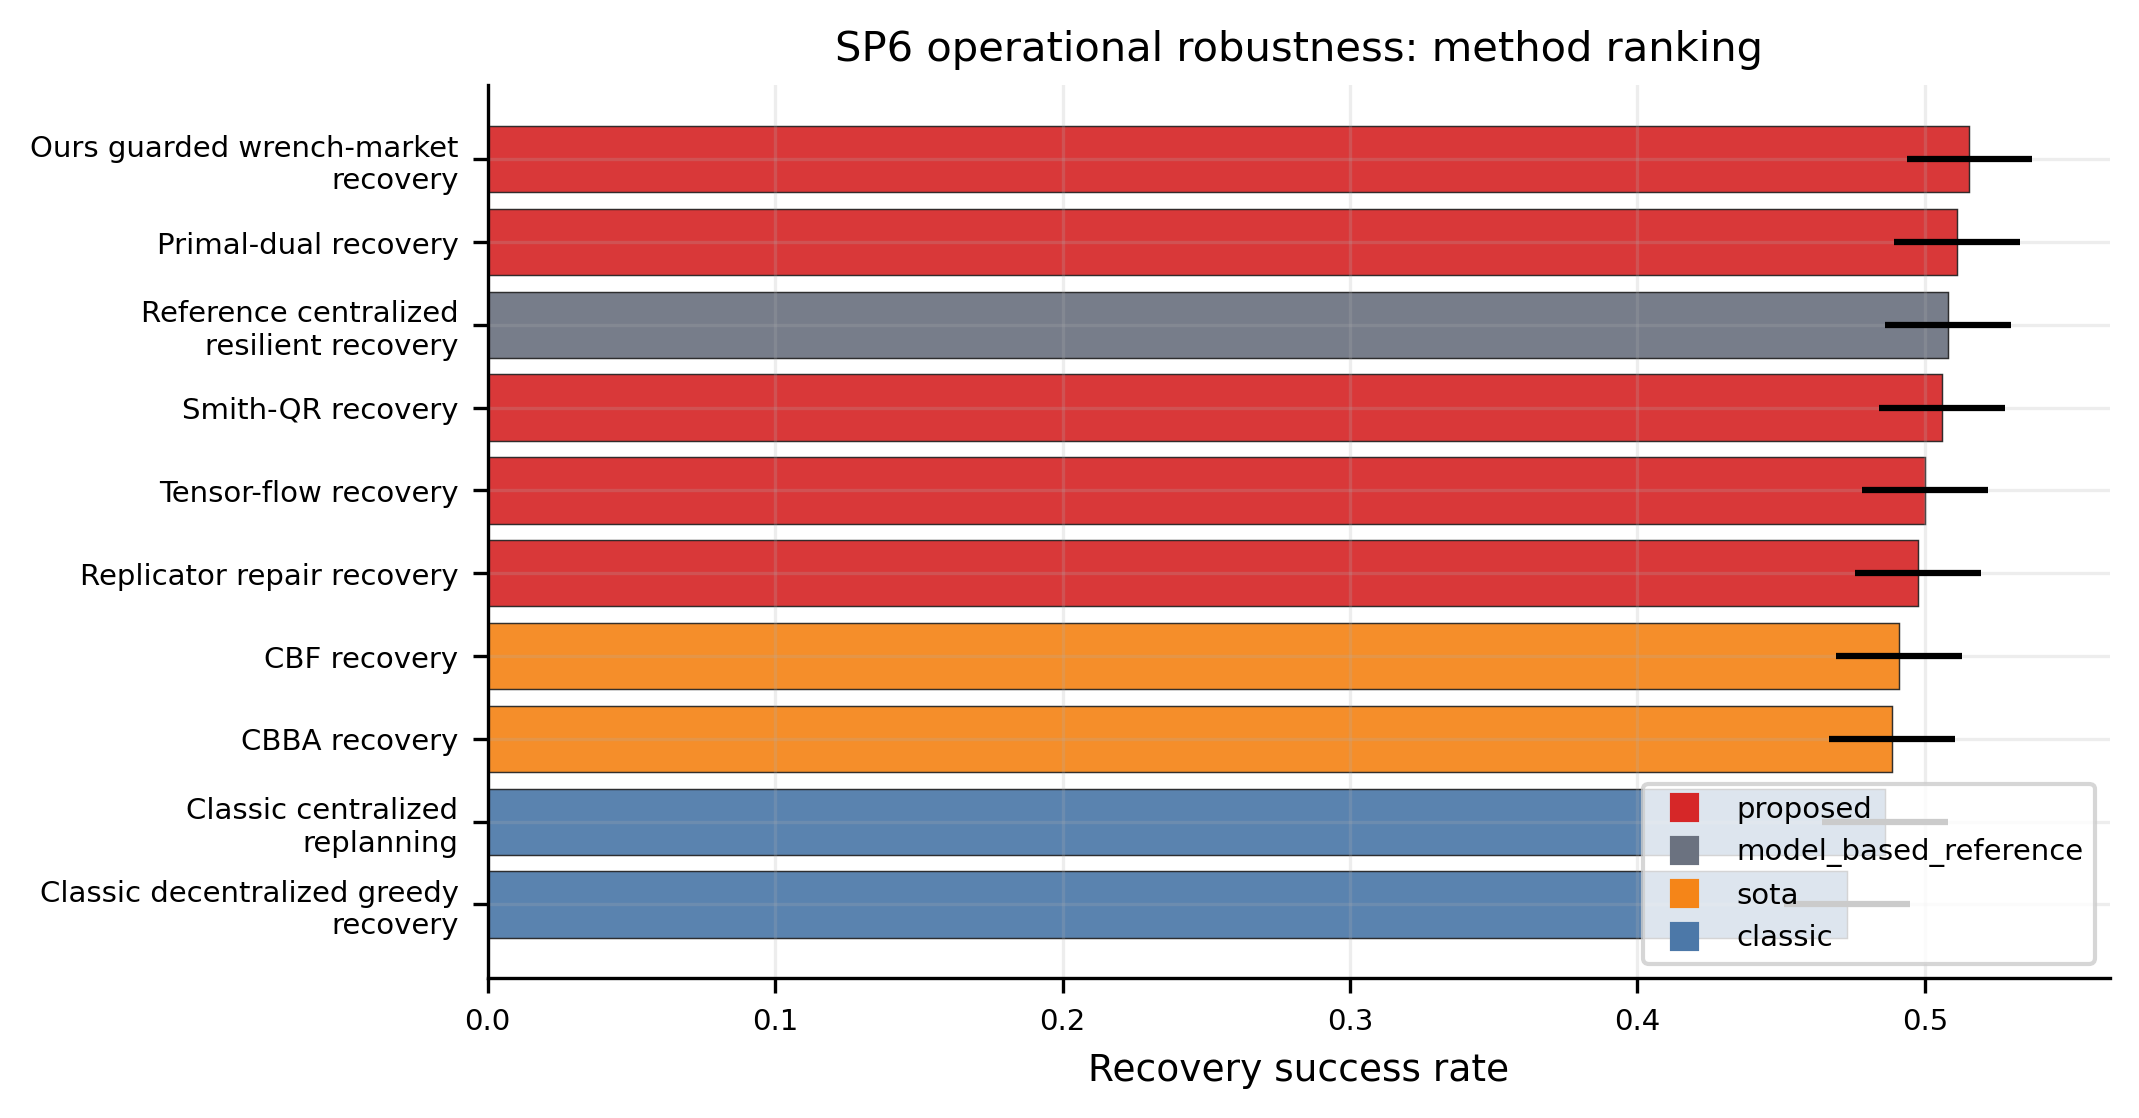
\includegraphics[width=0.74\textwidth]{figures/fig-sp6-primary.png}
\caption[Recuperación posterior a eventos en SP6]{La guardia posterior al
evento reduce pérdidas sin demostrar dominio global de completitud.}
\viuownsource
\label{fig:sp6-primary}
\end{figure}

La guardia de SP6 evita reparaciones que conservarían una carga inviable, pero su efecto aparece en pérdida y brecha, no en dominio global de la misión. En conjunto, SP4--SP6 muestran que una coalición estáticamente válida todavía puede fallar por trayectoria, pose o evento. También explican por qué A0--FULL debe evaluar la ejecución sobre la misma planta en lugar de sumar tasas procedentes de simuladores distintos.

\subsubsection{Fronteras no confirmatorias: SP7--SP8}

\paragraph{SP7: red observada, pero no inyectada en el lazo.}
SP7 reúne 20.176 filas sobre perfiles de comunicación y sensado. La correlación entre radio y conectividad temporal fue $\rho=0{,}8934$, pero las filas repiten mundos entre método y perfil. Además, pérdida, retardo y \emph{jitter} modifican registros o parámetros agregados; no existe una cola que altere en cada paso el estado vecino de un controlador fijo. La asociación se conserva como diagnóstico. H7.3 tiene $n_{\rm bloques}=0$ y se declara \textbf{no estimable}; el valor heredado $p=1$ no sustenta una conclusión nula.

\paragraph{SP8: escala mesoscópica sin medición común de recursos.}
SP8 representa flotas de $N=5$ a $N=50\,000$ mediante variables agregadas por zona. En las salidas conservadas, el flujo tensorial alcanzó completitud $0{,}1561$ y el mercado jerárquico $0{,}1529$, frente a $0{,}0521$ de \emph{greedy}; estas diferencias pertenecen al generador mesoscópico. Los timeouts del húngaro y del oráculo fueron declarados por reglas del evaluador, y la memoria procede de fórmulas analíticas, no de wall-clock y RSS observados bajo un watchdog común.

Las afirmaciones de escalado de recursos basadas en timeout declarado y memoria analítica quedan suspendidas. Los contrastes de calidad almacenados (H8.2--H8.3) se consideran exploratorios pese a sus valores $p$. Una campaña confirmatoria deberá ejecutar los métodos bajo el mismo timeout externo, medir tiempo y RSS, conservar la censura y hacer ciego el evaluador a la identidad del método. SP7--SP8 cumplen una función útil en la narrativa: marcan qué evidencia falta para extender la coalición física a redes reales y flotas industriales; no refuerzan el resultado integrado por acumulación de filas.
